% Все важные комментарии относительно кода помечены метками TODO или FIXME.
% Краткая справка по LaTeX: все комментарии начинаются с символа %, если таковой не нужно считать комментарием, он экранируется.
% Вся верстка зависит от DocumentClass'а и пакетов.
% Начало нового абзаца - пропуск строки.

%%%%%%%%
% В дальнейшем, буду давать некоторые комментарии, в местах где есть всевозможные странности, например где было сложно собрать достоверную информацию
%

\documentclass[a4paper,14pt,bachelor]{disser}
\usepackage{pscyr} % Шрифт Times New Roman
%\usepackage{cmlgc}
\usepackage{cmap}
\usepackage{mathtext, textcomp}
\usepackage[pdftex,unicode]{hyperref} % Красивые ссылки в pdf'ах, но возможны расхождения на +- страницу
\usepackage{fullpage}
\usepackage[left=20mm,right=10mm,top=20mm,bottom=20mm,headsep=0pt]{geometry} % Геометрия отступов, в мм
\usepackage[T2A]{fontenc} % Шрифт и кодировка
\usepackage[utf8]{inputenc}
\usepackage[english,russian]{babel} % Поддержка стандартных русских элементов типа неразрывного дефиса и т.д.
\usepackage{multirow} % возможность склеивать не только столбцы, но и строки
\usepackage{indentfirst} % Отступ в начале параграфа
\usepackage{amssymb,amsfonts,amsmath,amstext,enumerate,float,listings,longtable} % кучи вещей для цитатЙ, красивых листингов, разрывных таблиц, математических формул и символов
\usepackage{wrapfig} % обтекание текстов рисунков, врядли будет использоваться
\usepackage{bytefield} % Битовые карты, мб понадобится
\usepackage{hyperref}
\usepackage{hangcaption}
%\usepackage[small]{caption}
\usepackage{totcount}
\usepackage{lastpage} % Макрос lastpage, который дает ссылку и номер последней страницы
\pdfcompresslevel=9

\usepackage{graphicx} % картинки
\setkeys{Gin}{width=0.90\textwidth}
\graphicspath{{images/}} % Где их искать

\usepackage{pdfpages}
%\usepackage{cite}
\usepackage{bytefield}

%BEGIN Workarounds for disser style to conform MEPHI's requiments
\setcounter{tocdepth}{2} % В оглавлении два уровня вложенности - т.е. главы, секции и подсекции
% Далее несколько костылей, чтобы в стиле disser не проставлялись лишние точки или переводы строк в названиях глав.
\renewcommand\appendixalign{}
\renewcommand\appendixalign{}
\renewcommand\thechapteralign{}
\renewcommand\chapteralign{}
\renewcommand\postthechapter{\tocfill{.}}
\renewcommand\tocpostthechapter{\@postskip}
\renewcommand\captionfont{\centering\footnotesize}
\renewcommand\captionlabelfont{\captionfont\selectfont}
\renewcommand\tocprethechapter{~}
\renewcommand\prethechapter{\protect~}
\renewcommand\tocpostthechapter{\@postskip}
\renewcommand\tocpostthesection{\@postskip}
\renewcommand\postthesection{~}
\renewcommand\tocpostthesubsection{\@postskip}
\renewcommand\tocpostthesubsubsection{\@postskip}
\renewcommand\postthesubsubsection{~}
\renewcommand\tocpostthepart{}
\renewcommand\tocpostthechapter{}
\renewcommand\tocpostthesection{}
\renewcommand\tocpostthesubsection{}
\renewcommand\tocpostthesubsubsection{}
\renewcommand\postthepart{}
\renewcommand\postthechapter{\protect~}
\renewcommand\postthesection{\protect~}
\renewcommand\postthesubsection{\protect~}
\renewcommand\postthesubsubsection{\protect~}

% Более правильные заголовки у таблиц и подписи рисунков.
\long\def\@makecaption#1#2{%
  \vskip\abovecaptionskip
  \sbox\@tempboxa{{\captionlabelfont #1\captionlabeldelim} {\captionfont #2}}%
  \ifdim \wd\@tempboxa >\hsize
    {{\captionlabelfont  #1\captionlabeldelim} {\captionfont #2}}\par
  \else
    \global \@minipagefalse
    \hb@xt@\hsize{\hfil\box\@tempboxa\hfil}%
  \fi
  \vskip\belowcaptionskip
}

%END OF WORKAROUND

% Параметры для генерации титульного листа
\institution{Министерство образования и науки Российской федерации государственное бюджетное образовательное учреждение высшего профессионального образования <<Национальный исследовательский ядерный университет <<МИФИ>>}
\title{Пояснительная записка к дипломному проекту}
\topic{Разработка тестового программного обеспечения для процессорных модулей на базе микропроцессора NetX~500}
\author{Смирнов~В.Ю.}
\city{Москва}
\sa{ассистент каф. 27, Тихонов~Ю.Н.}
\group{А12-11}
\apname{д.т.н.,~Першенков~В.С.}
\rev{ст. преп. каф. 26, Азаров~Д.А.}

\lstset{
language=C,
basicstyle=\small\sffamily,
numbers=left,
numberstyle=\small\color{gray},
xleftmargin=80pt,
frame=single,
columns=fullflexible,
showstringspaces=false
}

\renewcommand{\lstlistingname}{Вставка}
\renewcommand{\lstlistlistingname}{\addcontentsline{toc}{chapter}{Список вставок}Список вставок}

\lstdefinelanguage[arm]{Assembler}%
  {morekeywords={ip,sp,r0,r1,r2,r3,r4,r5,r6,r7,r8,r9,r10,r11,r12,r13,r14,r15,
	  fp, mov, stmfd,sub,ldr,b,cmb,bcs,cmp,bcc,str,lr,pc, add, beq, lbs,
	  ldmfd, bls
},%
   morekeywords=[2]{.align},%
   alsoletter=.,alsodigit=?,%
   sensitive=f,%
   morestring=[b]",%
   morestring=[b]',%
   morecomment=[l];%
   }[keywords,comments,strings]

%\renewcommand{\baselinestretch}{1.65} % Если раскоентировать, получится примерно двойной отступ
\tolerance=10000 % запретить выходить за поля
%\pretolerance=10000 % если раскоментить, то переносы вообще исчезнут и текст начнет растягиваться всегда на всю ширину

%Уменьшаем шрифт во вставках.
\makeatletter
\def\verbatim@font{\small\ttfamily}
\makeatother
% Счетчики фигур и таблиц, т.к. не все нужно учитывать, да и стиль с total подглюкивает и выдает нули всегда на некоторые счетичики
\newtotcounter{myfigs}
\newtotcounter{tbls}
%BEGIN REAL DOCUMENT
% Начало самого документа.

\begin{document}

\maketitle % Делаем титульник
\setcounter{page}{2} % Говорим что следующая страница №2, в некоторых стилях она имеет №1
\chapter*{Аннотация} % глава, не попадающая в оглавление
Данная работа посвящена проектированию и разработке тестового программного обеспечения для процессорных модулей на базе микропроцессора NetX 500. Работа состоит из введения, трех глав и заключения. Общий объем работы \pageref{LastPage} страниц, \total{myfigs} рисунков и \total{tbls} таблиц.

\tableofcontents{} % оглавление
%\listoffigures % список рисунков
%\listoftables % список таблиц
%\lstlistoflistings

\chapter{Введение}
В развитии современных автоматизированных систем управления технологическим процессом (АСУ ТП) наблюдается тенденция перехода к модульной архитектуре, разделению всего комплекса на небольшие составные части, объединенные с помощью различных шин в единую систему. Увеличение мощности современных микропроцессоров и микроконтроллеров, а также переход от параллельных шин к высокоскоростным последовательным, позволяет создавать более надежные, распределенные АСУ ТП. Примером таких систем могут служить комплексы программно-технических средств ТПТС, разрабатываемые ФГУП ВНИИА им. Духова, используемые на ряде российских электростанций.

В настоящее время во ВНИИА ведутся работы по созданию нового поколения комплексов ТПТС -- ТПТС-НТ, отличительной особенностью которых является перераспределение функций автоматизации между компонентами системы. Основной задачей подобных изменений является обеспечение времени реакции системы на события в пределах 200 мс, предоставление возможности решения локальных задач с повышенными требованиями ко времени реакции (до 10мс), создание возможности распределения аппаратуры по объекту автоматизации, сокращение цикла изменения унифицированных аналоговых сигналов и улучшение фильтрации фильтрации измеряемых параметров. Структура комплекса ТПТС-НТ показана на рисунке \ref{tpts-main} % ссылка на рисунок, который будет ниже.

Программно-технические средства нового поколения включают в себя:
\begin{itemize}
 \item Коммуникационные средства для различных шин данных.
 \item Служебные модули для организации питания и сигнализации.
 \item Серверы автоматизации -- центральные модули, выполняющие прикладную программу, задачи приема-передачи данных по различным шинам.
 \item Станции ввода-вывода, состоящие из модулей связи с процессом и интерфейсных модулей.
\end{itemize}

\begin{figure}[h!] % вставляем рисунок.
\addtocounter{myfigs}{1}
 \begin{center}
 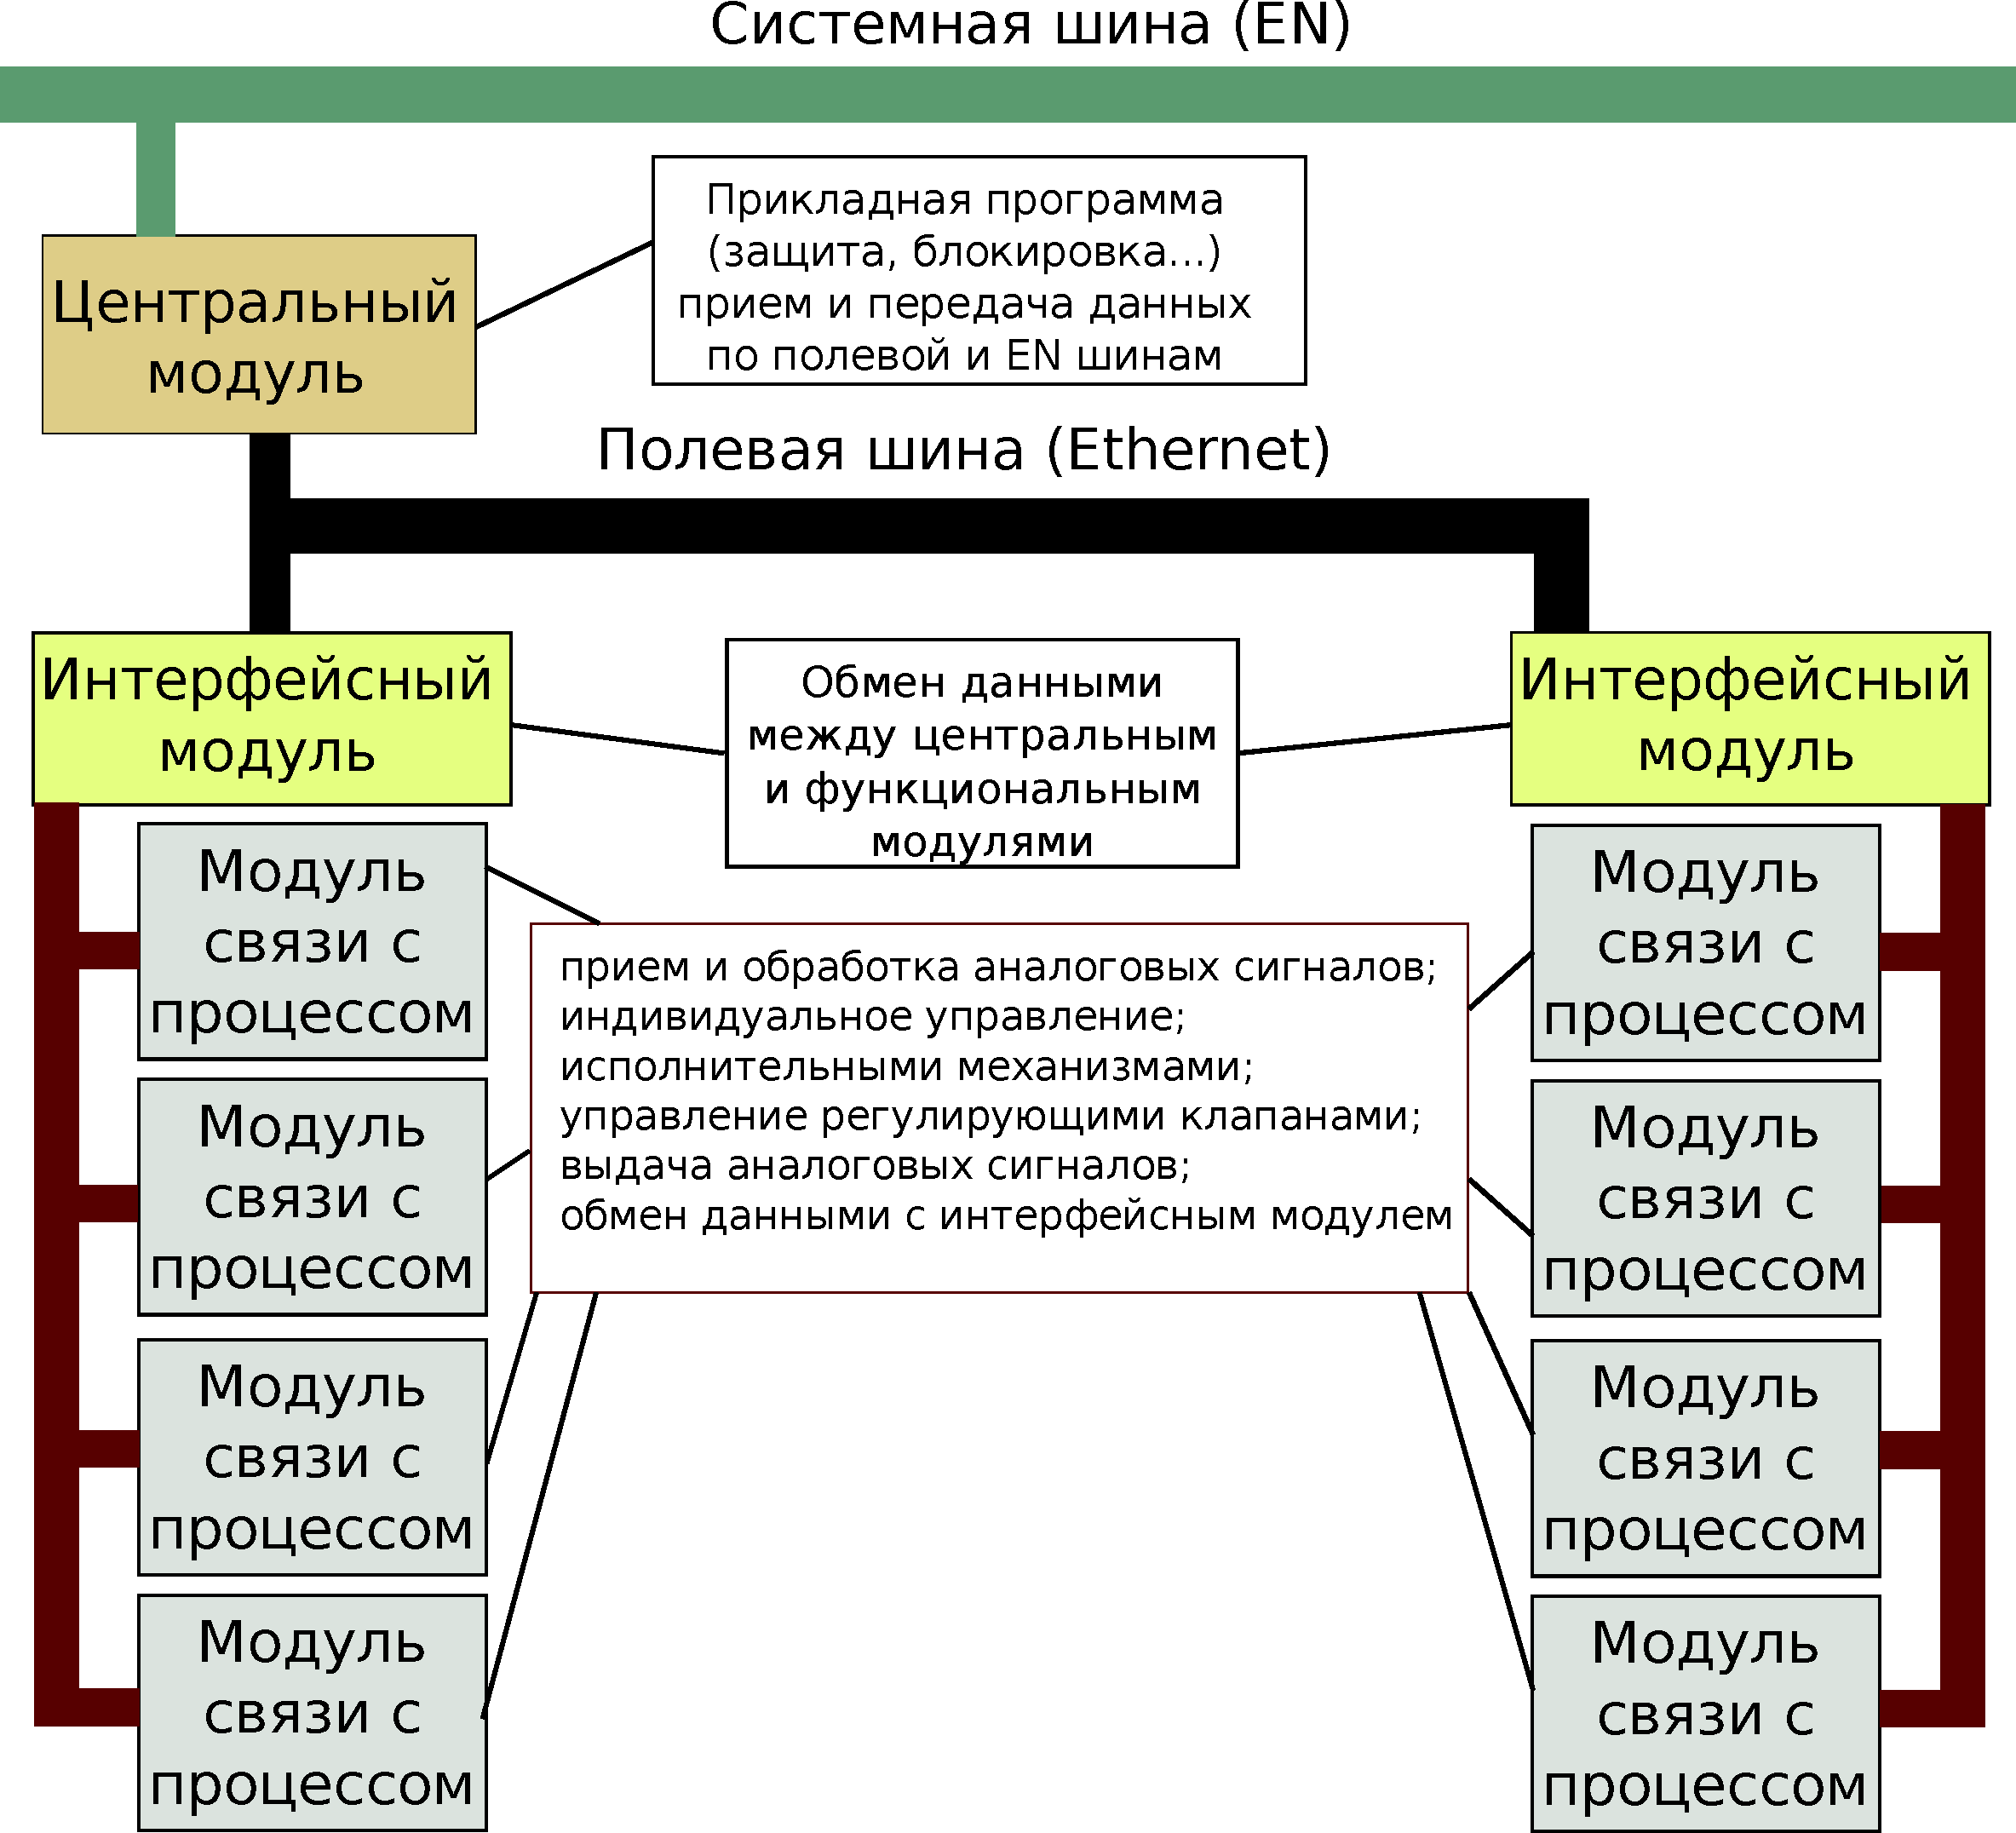
\includegraphics[width=0.7\textwidth]{tpts-nt}
 \caption{\label{tpts-main} Структура комплекса программно-технических средств ТПТС-НТ}
 \end{center}
\end{figure}

Базовые параметризуемые функции, характерные для всех объектов управления, хранятся в модулях самого нижнего уровня -- модулях связи с процессом. Модули связи с процессом не являются свободнопрограммируемыми и выполняют строго отведенные для них задачи, такие как измерение, фильтрацию входных данных, прием дискретных сигналов и т.п.

Прикладные программы, специфичные для каждого объекта автоматизации, программируемые проектировщиком, находятся в центральном модуле -- сервере автоматизации. Он выполняет определяемые проектом задачи, связанные с автоматическим управлением: технологические защиты, блокировки, расчетные задачи и т.п.

Такой подход к разделению модулей по функциональному назначению, позволяет использовать специализированные микропроцессоры в модулях связи, чтобы обеспечить минимальное время реакции системы на какие-либо изменения состояния технологического процесса, при этом, все сложные вычисления происходят на стороне более производительного сервера автоматизации, построенного на базе процессоров общего назначения.

Использование сервера автоматизации при построении систем безопасности, работающих в жестких условиях (температура окружающей среды может находится в диапазоне от $-40$ до $+85^\circ$C) исключает возможность использования IBM PC-совместимых компьютеров, а высокие требования к времени реакции на события исключают возможность использования операционных систем общего назначения. Поэтому, каждый конкретный модуль, проектируется на базе специальных микропроцессоров и микроконтроллеров. В качестве основы для коммуникационного модуля ТПТС55.1205 применяется ARM9-совместимый процессор Hilscher~NetX~500, а в качестве операционной системы - ОСРВ rcX.

Целью данной дипломной работы является разработка тестового программного обеспечения для коммуникационного модуля ТПТС55.1205, обеспечивающего взаимодействие компонентов сервера автоматизации с периферийными устройствами по шине PROFIBUS-DP. При выполнении дипломной работы решались следующие задачи:
\begin{enumerate}
 \item Разработка и реализация алгоритмов самотестирования.
 \item Разработка и реализация алгоритмов производственного тестирования.
 \item Разработка тестового комплекса для тестирования и верификации модуля.
\end{enumerate}

\chapter{Коммуникационные решения компании Hilscher}
\section{Микропроцессоры семейства NetX компании Hilscher}
% Комментарий: данные hilscher расходятся по каждому из процессоров даже в пределах одной страницы, например про NetX~50 Они в сводных характеристиках пишут, что он имеет 112КБ SRAM, а чуть ниже - 96. Скорее всего они посчитали SRAM + Cache, что несколько не правильно. Также про NetX~100 тоже характеристики расходятся - в общих они скопированы из NetX~500, включая поддержку RTOS и интерфейс для LCD-дисплеев, но при этом в описании сказано, LCD и RTOS особенность NetX~500 и в NetX~100 отсутствуют (также сказано в презентациях). Про количество контроллеров тоже есть расхождения - на схеме NetX~100 их подписано 3 (2 Ethernet/Fieldbus, 1 Fieldbus), но нарисовано 4 блока и т.п., далее попытка собрать всю информацию и выделить наиболее правдоподобное и интересное с точки зрения дипломной работы (обоснования выбора NetX~500 вместо NetX~100). Ориентировался в основном на netx_design_auswahl + блок-схемы с той страницы.
Компания Hilscher специализируется на производстве коммуникационных микропроцессоров и предлагает ряд решений для различных задач:
\begin{itemize}
 \item NetX~50 -- коммуникационный 32-х разрядный микропроцессор начального уровня на базе ядра ARM966E-S. Его ключевыми особенностями является отсутствие необходимости во внешнем кварцевом генераторе частоты, при условии что не будет использоваться внешняя SDRAM память, и отсутствие блока управления памятью (MMU).
 \item NetX~100 -- коммуникационный 32-х разрядный микропроцессор среднего уровня на базе ядра ARM926EJ-S, с поддержкой ускорения программ, написанных на языке Java (технология Jazelle DBX), поддержкой большего количества программируемых выходных каналов и с блоком управления памятью.
 \item NetX~500 -- коммуникационный 32-х разрядный микропроцессор для задач, требующих гарантированное время реакции на события. От предыдущего отличается количеством интерфейсов, объемом встроенной оперативной памяти SRAM и поддержкой операционных систем реального времени RTLinux, rcX и VxWorks, при этом ядро ОСРВ rcX находится во встроенной ROM процессора.
\end{itemize}



Все микропроцессоры семейства NetX соответствуют индустриальным стандартам по допустимым рабочим условиям -- диапазон рабочих температур, при условии использования пассивного охлаждения, составляет -40$^o$--85$^o$C.

Сравнительная характеристика процессоров представлена в таблице \ref{netx-comparation}.

\begin{center}
\addtocounter{tbls}{1}
\begin{longtable}{|c|c|c|c|}
\caption{\label{netx-comparation}Сравнительная характеристика коммуникационных микропроцессоров компании Hilscher}\\
\hline & NetX~50 & NetX~100 & NetX~500 \\\hline
\endfirsthead
\multicolumn{4}{c}{Продолжение таблицы \thetable}
\endhead
Дата выпуска & \multicolumn{3}{|c|}{2005 г.} \\\hline
Архитектура & \multicolumn{3}{|c|}{ARM9} \\\hline
Ядро & ARM966E-S & \multicolumn{2}{|c|}{ARM926EJ-S} \\\hline
Частота & \multicolumn{3}{|c|}{200МГц} \\\hline
Кэш-память & 0КБ & 24 КБ & 24 КБ \\\hline
Коммуникационные каналы & 2 & 3 & 4 \\\hline
Объем встроенной RAM & 96КБ & 144КБ & 144КБ \\\hline
Поддержка DP-RAM & 32КБ & \multicolumn{2}{|c|}{64КБ} \\\hline
ROM & 64КБ & \multicolumn{2}{|c|}{32КБ} \\\hline
Поддержка запуска ОСРВ & нет & нет & да \\\hline
Энергопотребление & 0.8-1.2Вт & 1.0-1.5Вт & 1.0-1.5Вт \\\hline
\end{longtable}
\end{center}

\subsection{NetX~50}
По своим характеристикам, данный микропроцессор больше похож на 32-х разрядные микроконтроллеры. Отсутствие блока управления памятью исключает возможность работы современных многозадачных встраиваемых операционных систем, таких как Linux или Windows CE. Существуют проекты по запуску Linux на устройствах без MMU, но они не гарантируют стабильной бесперебойной работы и, поэтому, на данный момент не подходят для ответственных применений. Блок управления памяти выполняет преобразование виртуальных адресов в физические, а это необходимо для любой многозадачной операционной системы.

Также, данный процессор содержит два универсальных программируемых коммуникационных канала, называемых в данной серии процессоров xPEC. Оба блока реализуют физический уровень RS485 и Ethernet. Особенностью xPEC является возможность перепрограммировать его на поддержку практически любого протокола, в таком случаи останется реализовать только физический уровень или использовать имеющуюся реализацию Ethernet или RS-485.

Компания Hilscher рекомендует использовать данный процессор для реализации простых преобразователей данных между двумя протоколами с возможностью минимальной обработки сигналов. Отсутствие MMU и кэшей делают использование данного процессора в высокопроизводительных средах затруднительными. Его следует рассматривать больше как высокопроизводительный 32-х разрядный микроконтроллер с ARM-совместимым ядром, нежели как микропроцессор.

Из-за всех перечисленных недостатков, данный процессор не подходит на роль центрального процессора в коммуникационной плате сервера автоматизации.

\subsection{NetX~100}
В отличии от NetX~50, данный процессор построен на базе ядра ARM926EJ-S, поэтому обладает MMU и 24КБ кэш-памяти (8КБ для инструкций, 16КБ для данных). Это позволяет запускать на данном процессоре полноценные операционные системы, такие как Linux или Windows CE.

Данный процессор обладает тремя программируемыми коммуникационными каналами. У третьего канала отсутствует блок физического уровня Ethernet. Встроенная оперативная память была расширена до 144КБайт, но ROM, при этом, сокращен до 32КБ.

Процессор NetX~100 рассчитан для работы в средах, где важна параллельное общение с несколькими каналами. При всем при этом, довольно существенным недостатком по сравнению с другими решениями серии NetX, является отсутствие доступной реализации стеков протоколов Fieldbus, Modbus, Ethernet и Profibus для какой либо из операционных систем, поддерживающих данный контроллер.

\subsection{NetX~500}
По своим характеристикам, данный процессор очень похож на NetX~100. Главным отличием является наличие 4-х программируемых коммуникационных каналов и дополнительного ROM, в котором содержится ядро операционной системы реального времени rcX, более подробную информацию о котором можно получить из \cite[Programming reference guide]{rcX}. Также данный процессор является единственным в линейке, который официально поддерживает работу с операционными системами реального времени, такими как VxWorks. Также под rcX и VxWorks доступен полный программный стек протоколов. Структурную схему процессора можно увидеть на рисунке \ref{netx500-scheme}.

\begin{figure}[h!] % вставляем рисунок.
\addtocounter{myfigs}{1}
 \begin{center}
 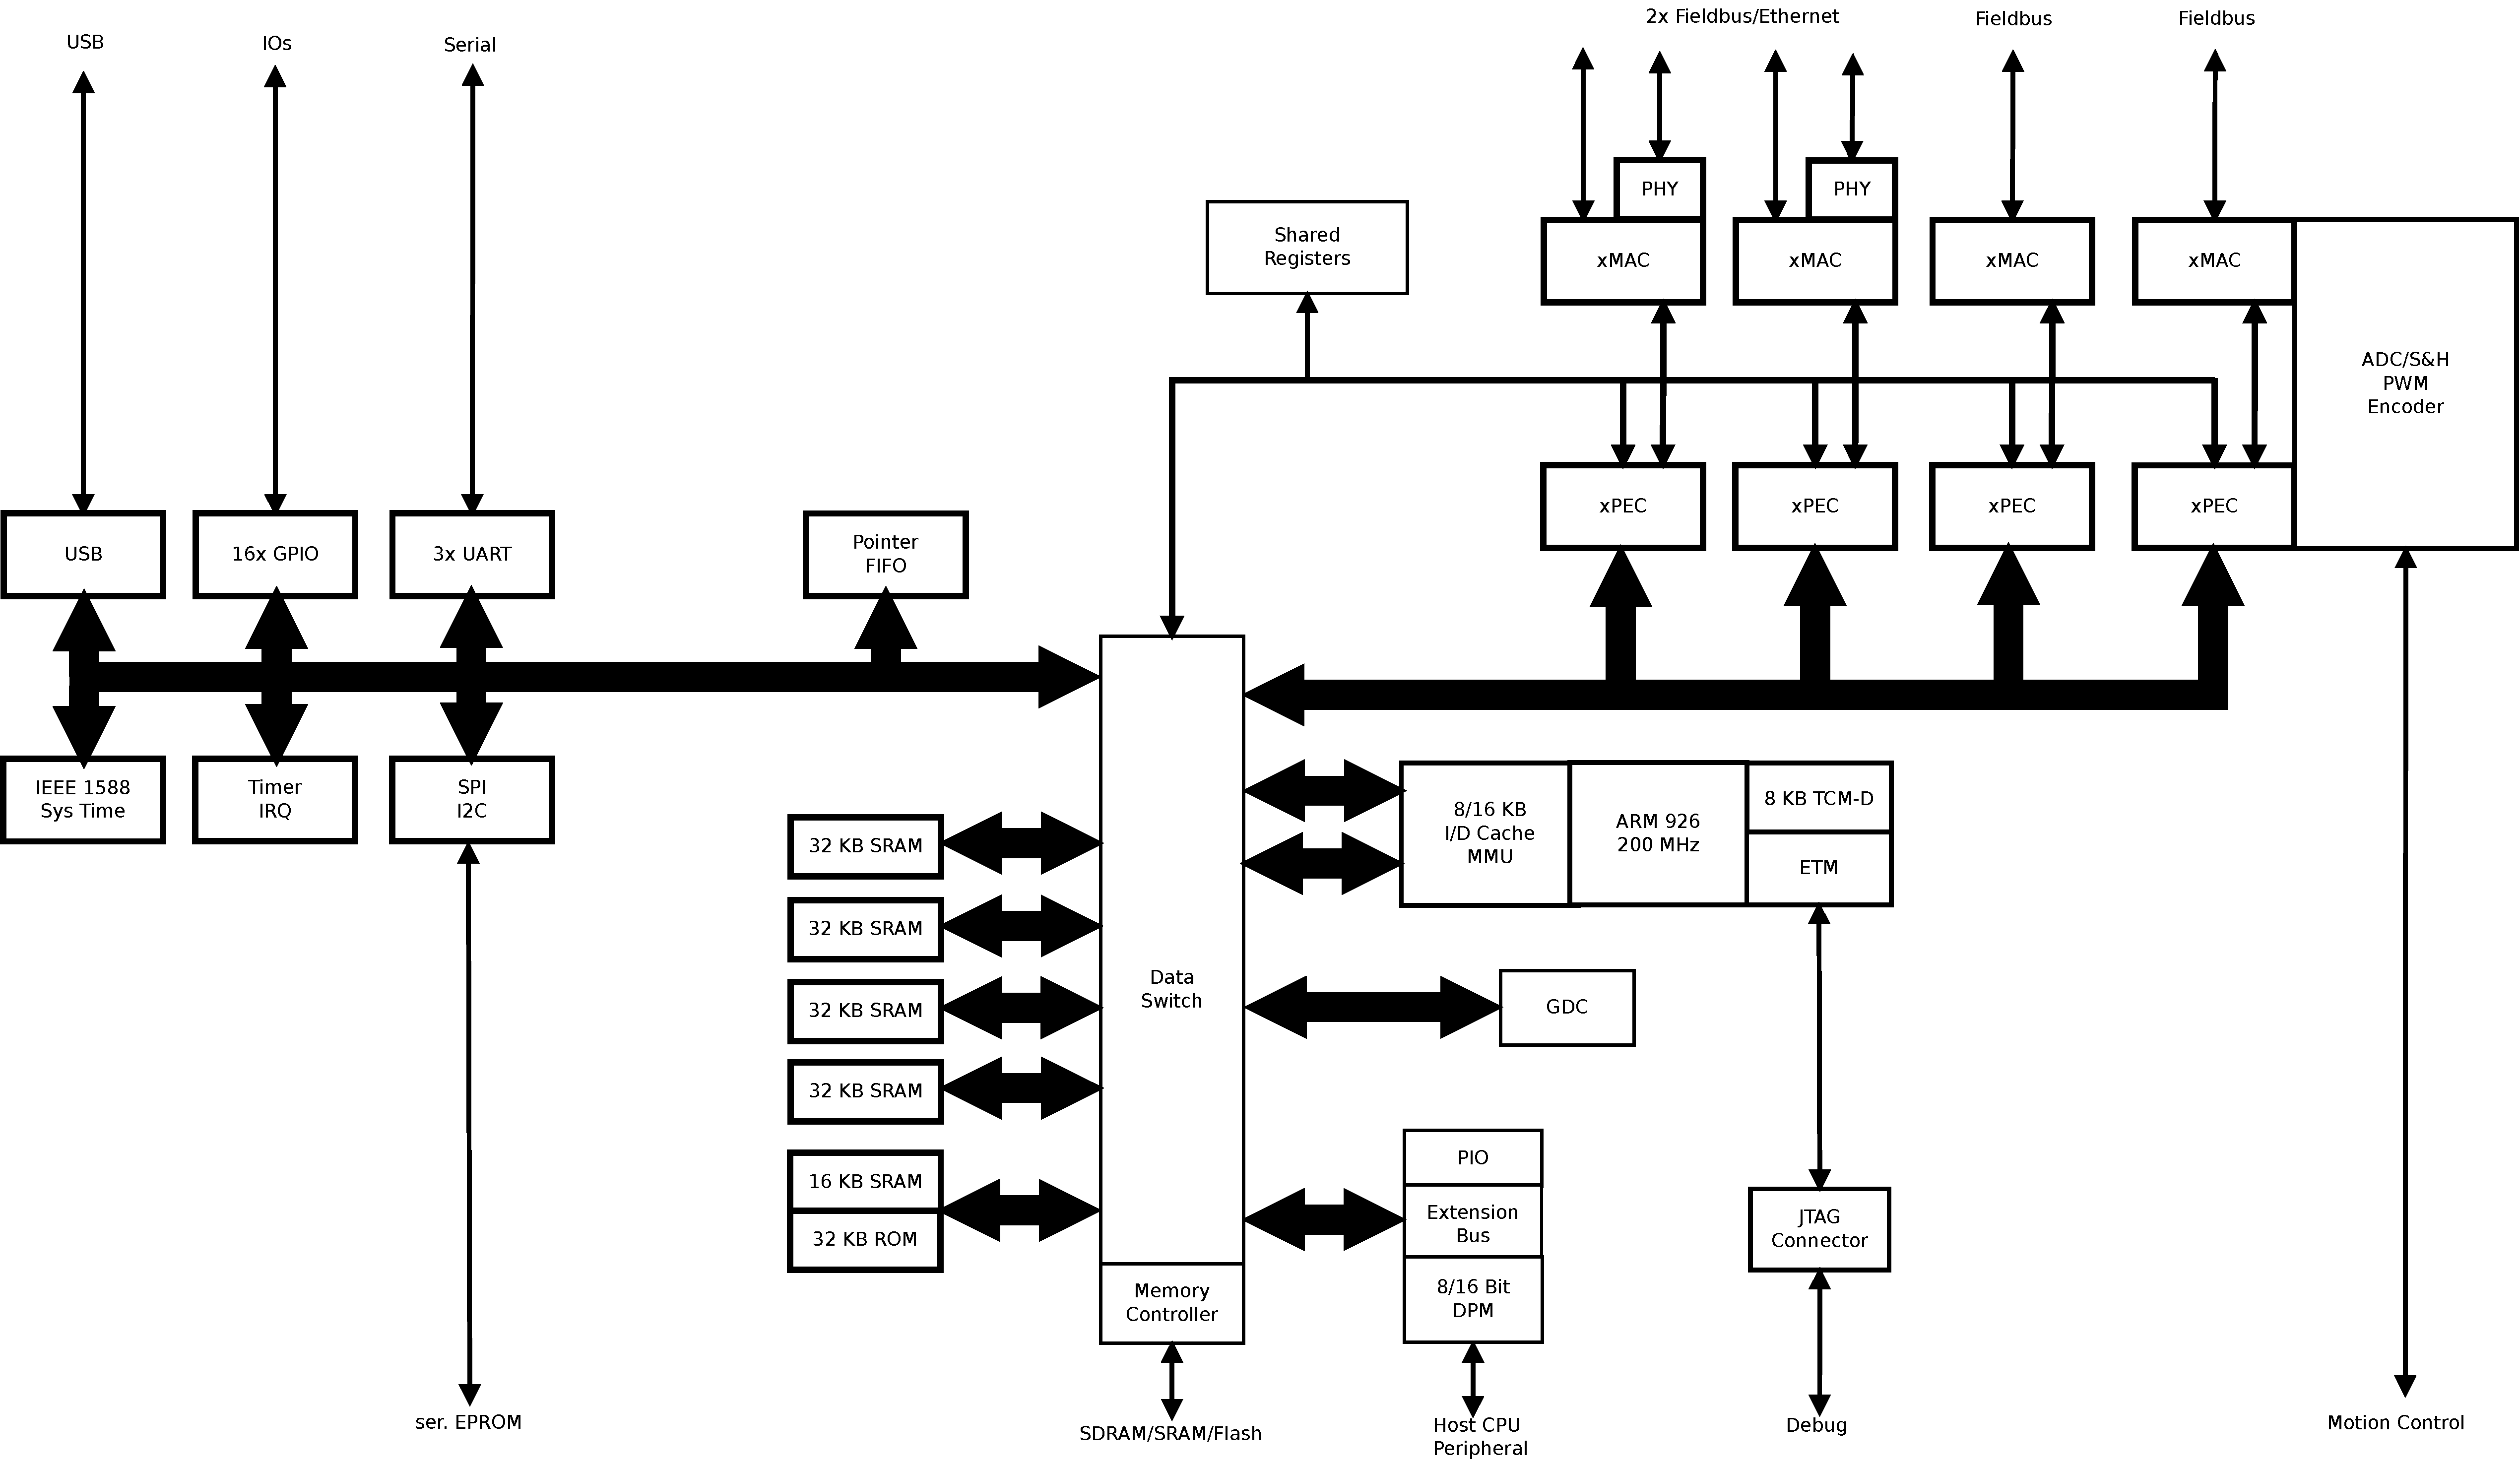
\includegraphics[width=0.9\textwidth]{netx500}
 \caption{\label{netx500-scheme} Структурная схема процессора NetX~500}
 \end{center}
\end{figure}

NetX~500 рассчитан на применение в устройствах, для которых важна гарантированная реакция на события. Таким образом, данный процессор больше других из этого семейства подходит для коммуникационной платы сервера автоматизации, применяемого в АСУ ТП электростанций.

\section{Программное обеспечение для процессоров NetX~500}
Компания Hilscher предлагает несколько основных типов программного обеспечения для своих процессоров. Его можно поделить на несколько различных классов:
\begin{itemize}
 \item Операционные системы.
 \item Демонстрационные примеры.
 \item Стеки протоколов.
 \item Прикладное программное обеспечение для разработчиков (отладчики, среды разработки, компиляторы).
\end{itemize}

\subsection{Операционные системы}
Микропроцессоры серии NetX компании Hilscher поддерживают запуск некоторых операционных систем, что позволяет упростить разработку программного обеспечения и получить заданные параметры времени реакции на внешние события.

Список операционных систем достаточно обширен и включает в себя такие ОС, как:
\begin{itemize}
 \item Linux
 \item Microsoft Windows CE
 \item RTLinux (Real-Time Linux)
 \item Windriver VxWorks
 \item Hilscher rcX
\end{itemize}

\subsubsection{Linux}
\begin{itemize}
 \item Операционная система общего назначения.
 \item Поддержка большого количества архитектур.
 \item Поддержка многоядерных систем.
 \item Совместима с POSIX.
 \item Большое количество различного программного обеспечения.
 \item Отсутствие реализаций стека протоколов для процессоров NetX.
 \item Гибкая конфигурация ядра ОС.
 \item Высокие требования к ресурсам: 2МБ флеш-памяти, 4МБ оперативной памяти.
\end{itemize}

Данная операционная система больше подходит для построения производительных пользовательских терминалов, нежели для использования в системах автоматизации.

\subsubsection{Windows CE}
\begin{itemize}
 \item Мягкое реальное время
 \item Вытесняющая многозадачность
 \item Модульная архитектура
 \item Оптимизирована под ARM-совместимые процессоры
 \item Высокие системные требования: от 1 Мбайта флеш-памяти, от 8МБ оперативной памяти
 \item Платная лицензия: от 3 до 16\$ за устройство.
\end{itemize}

Аналогично предыдущей, имеет смысл использовать данную ОС для построения терминалов.

\subsubsection{RTLinux}
\begin{itemize}
 \item Жесткого реального времени.
 \item Запускает практически немодифицированное ядро Linux как один из процессов.
 \item Поддержка большого количества архитектур.
 \item Поддержка многоядерных систем.
 \item Совместима с POSIX.
 \item Большое количество различного программного обеспечения.
 \item Большие задержки при выполнении задач.
 \item Отсутствие драйверов для периферийных интерфейсов связи процессора NetX.
 \item Гибкая конфигурация ядра ОС.
 \item Высокие требования к ресурсам: 2МБ флеш-памяти, 4МБ оперативной памяти.
\end{itemize}

В отличии от Linux, данная ОС гарантирует время отклика на внешние события, что позволяет, потенциально, использовать её в системах АСУ ТП. Однако, высокие системные требования и низкая скорость работы в целом, а также отсутствие значительной части драйверов, ограничивают полезную область применения данной ОС в комплексе ТПТС-НТ. RTLinux имеет смысл использовать при переходе с других POSIX-совместимых ОСРВ, при условии что объем и сложность написанного программного обеспечения превышает объем и сложность реализации драйверов для периферийных шин и устройств. Также возможно использование данной ОС в качестве основы для терминалов управления, входящих в состав АСУ ТП, так как под Linux существует достаточно большое количество различных графических приложений и средств разработки, цена на коммерческое использование которых крайне низкая или отсутствует.

\subsubsection{VxWorks}
\begin{itemize}
 \item Жесткое реальное время
 \item Микроядерная операционная система
 \item Совместимость с POSIX
 \item Поддержка различных процессорных архитектур
 \item Поддержка многоядерных систем.
 \item Низкие системные требования: от 80КБ флеш-памяти, от 20КБайт оперативной памяти.
 \item Доступен полный стек протоколов для NetX~500.
 \item Высокая стоимость: 7500\$/год за право разработки, 375\$/год за право выпуска устройств
\end{itemize}

Из-за высокой цены лицензирования, данную ОСРВ имеет смысл использовать только, если осуществляется переход с имеющегося оборудования под управлением VxWorks на новое, на базе NetX~500.

\subsubsection{rcX}
\begin{itemize}
 \item Жесткое реальное время
 \item Вытесняющая многозадачность
 \item Модульная архитектура
 \item Оптимизирована под ARM9-совместимые процессоры
 \item Высокая скорость выполнения операций.
 \item Низкие системные требования: ядро встроено в ROM процессора, минимальный размер программы меньше 1КБ. Для работы ОСРВ и прикладных программ достаточно менее чем 30КБ оперативной памяти.
 \item Бесплатная
\end{itemize}

Данную ОСРВ имеет смысл использовать, когда разработка под NetX~500 ведется с нуля. С одной стороны она обладает очень низкими системными требованиями, с другой является достаточно быстрой и модульной. Также для нее доступен полный стек протоколов, часть из которых поставляется в составе пакета поддержки (Board Support Package) вместе с процессорами семейства NetX.

\subsection{Стек протоколов}
Компания Hilscher предоставляет различные варианты реализации стека протоколов для всех шин, поддерживаемых процессором NetX~500. Предоставляются они в двух вариантах:
\begin{enumerate}
 \item Самостоятельные (stand-alone) приложения -- объектные модули, исходные коды или полноценные приложения, не требующие rcX.
 \item Системные и прикладные модули для rcX -- объектные модули или исходные коды драйверов, либо полноценные приложения, использующие rcX.
\end{enumerate}

Наличие готового стека протоколов позволяет компании-заказчику не заниматься разработкой драйверов самостоятельно, а купить готовый стек протоколов, который протестирован и верифицирован. Это также позволяет компании-заказчику сосредоточиться на реализации прикладного программного обеспечения, не тратя время на разработку, верификацию и сертификацию низкоуровневого программного обеспечения, обеспечивающего работу необходимых аппаратных интерфейсов.

\subsection{Среда разработки HiTOP Environment}
В комплекте с решениями компании Hilscher предоставляется интегрированная среда разработки HiTOP Environment. Интерфейс программы представлен на рисунке \ref{hitop}. В качестве основы, используется набор компиляторов GNU Compiler Collection (GCC) версии 4.3.3. Данный набор компиляторов полностью реализует стандарты ANSI C, ISO C89, ISO C90\ref{shildt}, ANSI C++, ISO C++98, частично реализует стандарт C99, а также имеет ряд отключаемых расширений для стандарта C90 (gnu90). Расширения gnu90 позволяющие использовать так возможности как поддержка inline-функций, дополнительных макросов, например макросов оптимизаций условий (likely/unlikely)\cite{Griffits}, а также расширенное управление распределением памяти, в частности возможность использовать конкретные регистры для размещения переменных.

\begin{figure}[h!] % вставляем рисунок.
\addtocounter{myfigs}{1}
 \begin{center}
 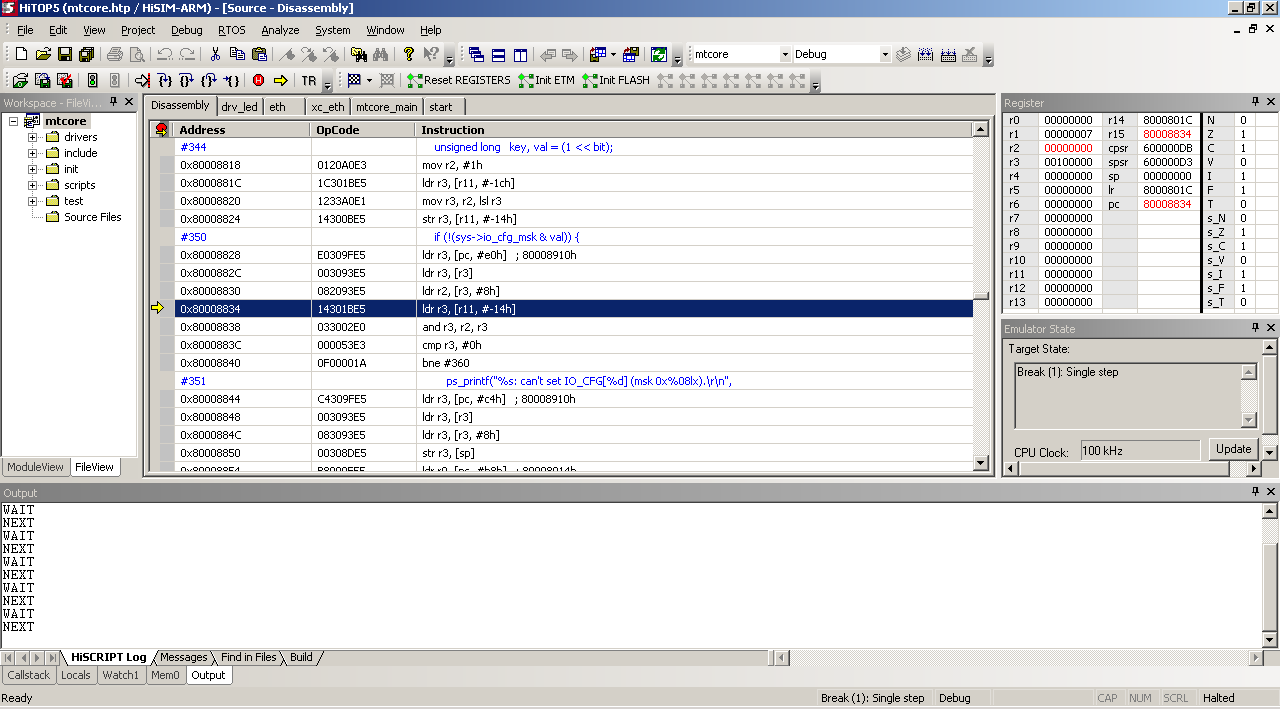
\includegraphics[width=0.9\textwidth]{hitop}
 \caption{\label{hitop} Интерфейс среды разработки}
 \end{center}
\end{figure}

Хотя языки C и C++ по своей сути являются переносимыми, но различные компиляторы могут реализовывать стандарт языка не в полной мере или трактовать некоторые неоднозначные места иначе, поэтому, в случаи переноса проекта на другую архитектуру, важным преимуществом является поддержка компиляторами GCC большого набора архитектур. В данной версии поддерживается 43 различных популярных процессорных архитектуры, например MIPS, Alpha, PowerPC, SPARC и т.д. Таким образом перенос проекта на любую другую архитектуру, поддерживаемую в GCC занимает минимальное время.

\section{Обзор альтернативных решений}
В техническом задании \cite{TZ}, утвержденном в 2008 году, к микропроцессору, лежащему в основе ТПТС55.1205, предъявляются следующие требования:
\begin{itemize}
 \item Объем двухпортовой памяти DP-RAM не менее 64КБ
 \item Наличие как минимум 1 порта Ethernet с поддержкой Real-Time Ethernet.
 \item Поддержка Profibus на скоростях до 1Мбита.
\end{itemize}

На тот момент, единственным микропроцессором, полностью удовлетворяющим всем предъявленным требованиям, являлся Hilscher~NetX~500. В рамках дипломной работы был проведен обзор альтернативных NetX~500 решений, доступных в данный момент, и были выявлены следующие микросхемы, наиболее близко отвечающие требованиям: Freescale~MPC8270\cite{Sheg}, Texas~Instruments AM1810. Сравнительная характеристика микросхем приведена в таблице \ref{netx-other-comparation}.

% И по FreeScale и по TI AM1810 некоторые данные были выяснены косвенным путем (не по даташитам и описаниям, а по каким-то рекламным презентациям, анонсам и т.п.). По Ti это техпроцесс и статус поддержки Profibus, по DPRAM там совсем непонятно, но из Datasheet'а я сделал вывод, что он его вообще не умеет. По Freescale -- энергопотребление, оно расходится в некоторых источниках. По NetX -- цена, на момент написания раздел на hilscher.com был недоступен.
\begin{center}
\addtocounter{tbls}{1}
\begin{longtable}{|p{5cm}|c|c|c|}
\caption{\label{netx-other-comparation}Сравнительная характеристика микропроцессоров NetX~500, MPC8270 и AM1810}\\
\endfirsthead
\multicolumn{4}{c}{Продолжение таблицы \thetable}
\endhead
\hline & NetX~500 & MPC8270 & AM1810 \\\hline
Дата выпуска & 2006 & 2008 & 2011 \\\hline
Архитектура & ARM9 & PowerPC & ARM9 \\\hline
Техпроцесс & 130нм & 130нм & 90нм \\\hline
Тактовая частота & 200MHz & 266MHz & 300МГц \\\hline
Частота системной шины & 100MHz & 66MHz & 100МГц \\\hline
Поддержка Profibus & 4 & 1 & 1, нужен трансивер \\\hline
USB & 1.1 & 1.1 & 2.0 \\\hline
DPRAM & 64КБ & 32КБ & - \\\hline
Энергопотребление & 1.5Вт & 2Вт & 0.7Вт \\\hline
Рабочие температуры & -40--85$^\circ$C & -40--85$^\circ$C & -40--105$^\circ$C \\\hline
Наличие готового ПО для стека протоколов & + & - & - \\\hline
Цена & 30\$ & 10\$ & 10\$ \\\hline
\end{longtable}
\end{center}

Из представленных в таблице микропроцессоров, под поставленные требования больше всего подходит Hilscher~NetX~500. Также, стоит отметить тот факт, что на момент составления технического задания, он был единственным доступным в продаже микропроцессором. 

\chapter{Тестируемые процессорные модули}
\section{Область применения}
Тестируемые процессорные модули входят в состав сервера автоматизации и выполняют роль связующего звена между сервером автоматизации и устройствами на шине Profibus. Для различных конфигураций сервера автоматизации выпускается два варианта модулей - ТПТС55.1205 и ТПТС55.1206.

С точки зрения сетевой модели OSI, отличие между процессорными модулями ТПТС55.1205 и ТПТС55.1206 ограничиваются физическим и канальным уровнем. Физическим уровнем для 1205 является RS485, а для 1206 таковым является RealTime-Ethernet. Канальный уровень 1205 реализует протокол Profibus, в то время как в 1206 используется Ethernet (стандарт IEEE 802.3). Формально, можно считать, что ТПТС55.1206 реализует связь с Profinet устройствами.

Блок-схему процессорных модулей можно увидеть на рисунке \ref{tpts_scheme}. Разработка аппаратной части процессорных модулей выполнялась на кафедре 26.

\begin{figure}[h!] % вставляем рисунок.
\addtocounter{myfigs}{1}
 \begin{center}
 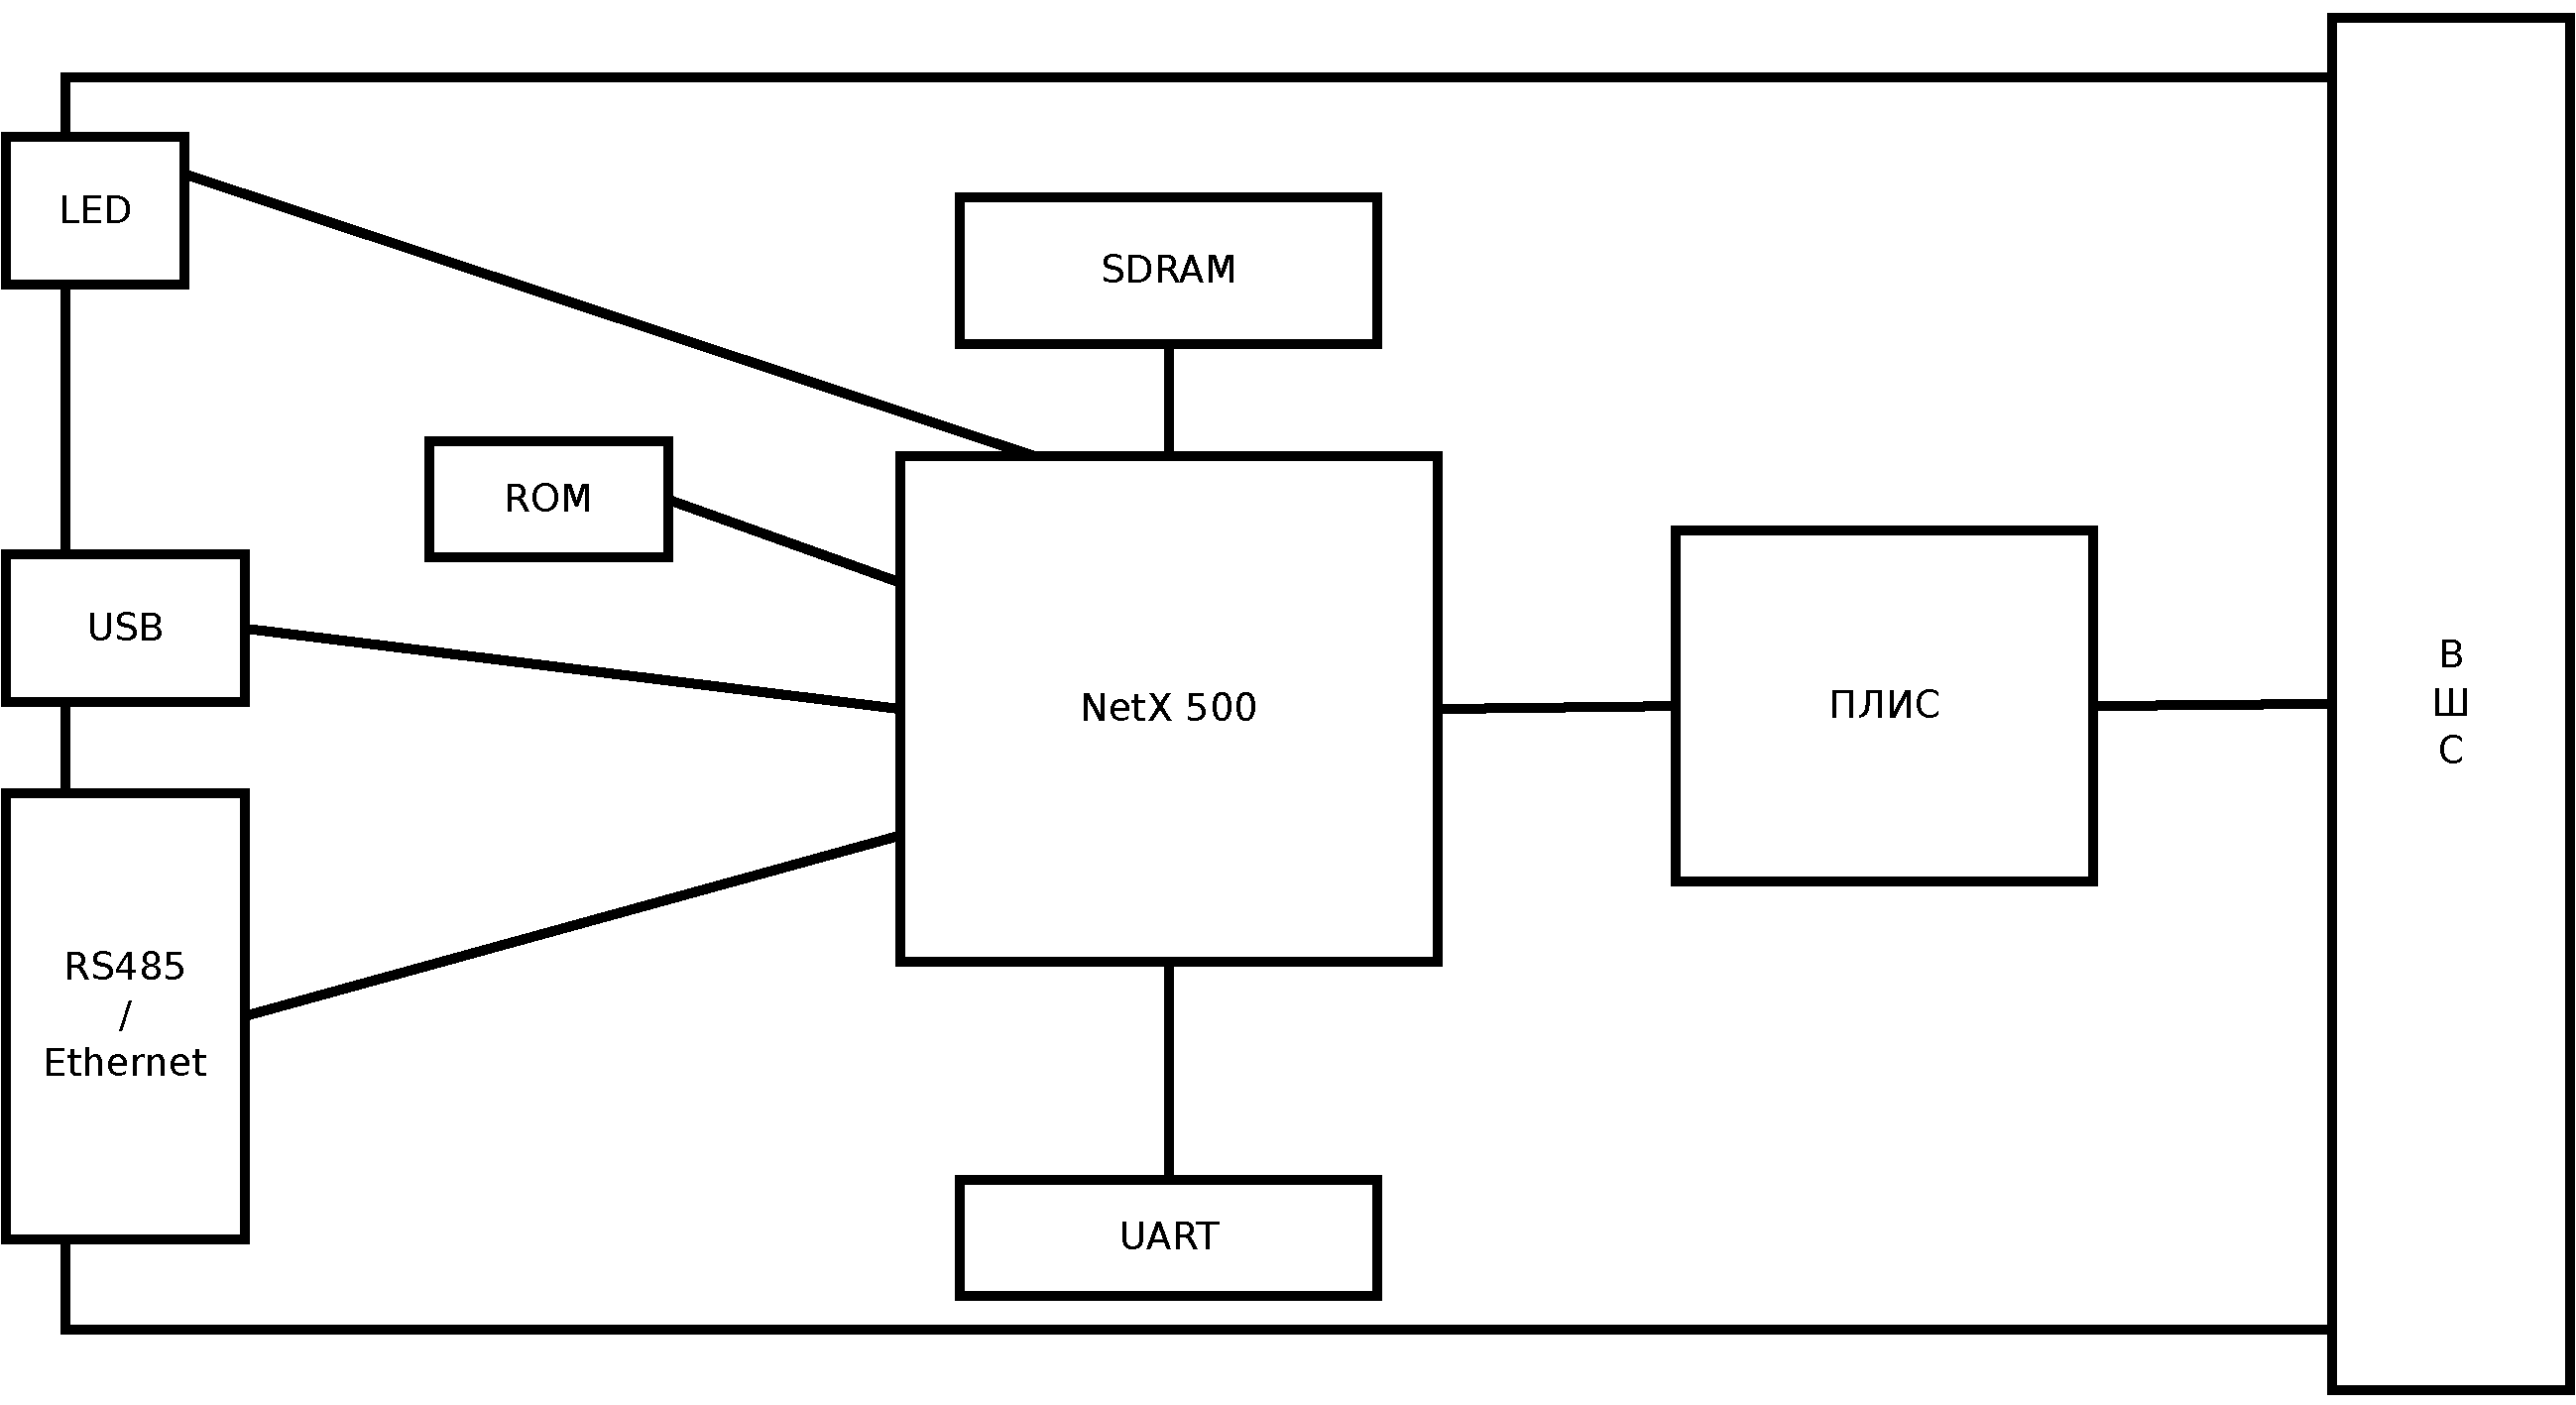
\includegraphics[width=0.9\textwidth]{tpts_scheme}
 \caption{\label{tpts_scheme} Блок-схема процессорных модулей ТПТС.1205/06}
 \end{center}
\end{figure}

\section{Технические характеристики}
Основные технические характеристики плат ТПТС55.1205/06 представлены в таблице \ref{tpts_tech}.

\begin{center}
\addtocounter{tbls}{1}
\begin{longtable}{|c|c|}
\caption{\label{tpts_tech}Технические характеристики плат ТПТС55.1205/06}\\
\hline Параметр & Значение \\\hline
\endfirsthead
\multicolumn{2}{c}{Продолжение таблицы \thetable}
\endhead
Процессор & NetX~500 \\\hline
Тактовая частота & 200МГц \\\hline
RAM & 16МБ SDRAM \\\hline
ROM & 2x4МБ SPI \\\hline
JTAG & 1 \\\hline
USB & 1 (host/client) \\\hline
COM & 2 \\\hline
ВШС & 1 \\\hline
Напряжение питания & 9-36 В \\\hline
\end{longtable}
\end{center}

В зависимости от модификации, возможно наличие либо разъемов Ethernet, либо разъема RS485 (Profibus).Внешний вид процессорной платы ТПТС55.1205 представлен на рисунке \ref{tpts_1205}. Передняя панель платы ТПТС55.1206 представлена на рисунке \ref{tpts_1206}

Процессорные модули содержат две микросхемы SPI Flash памяти модели Atmel AT45DB321D. Выбор используемой микросхемы ROM осуществляется перемычкой.

\begin{figure}[H] % вставляем рисунок.
\addtocounter{myfigs}{1}
 \begin{center}
 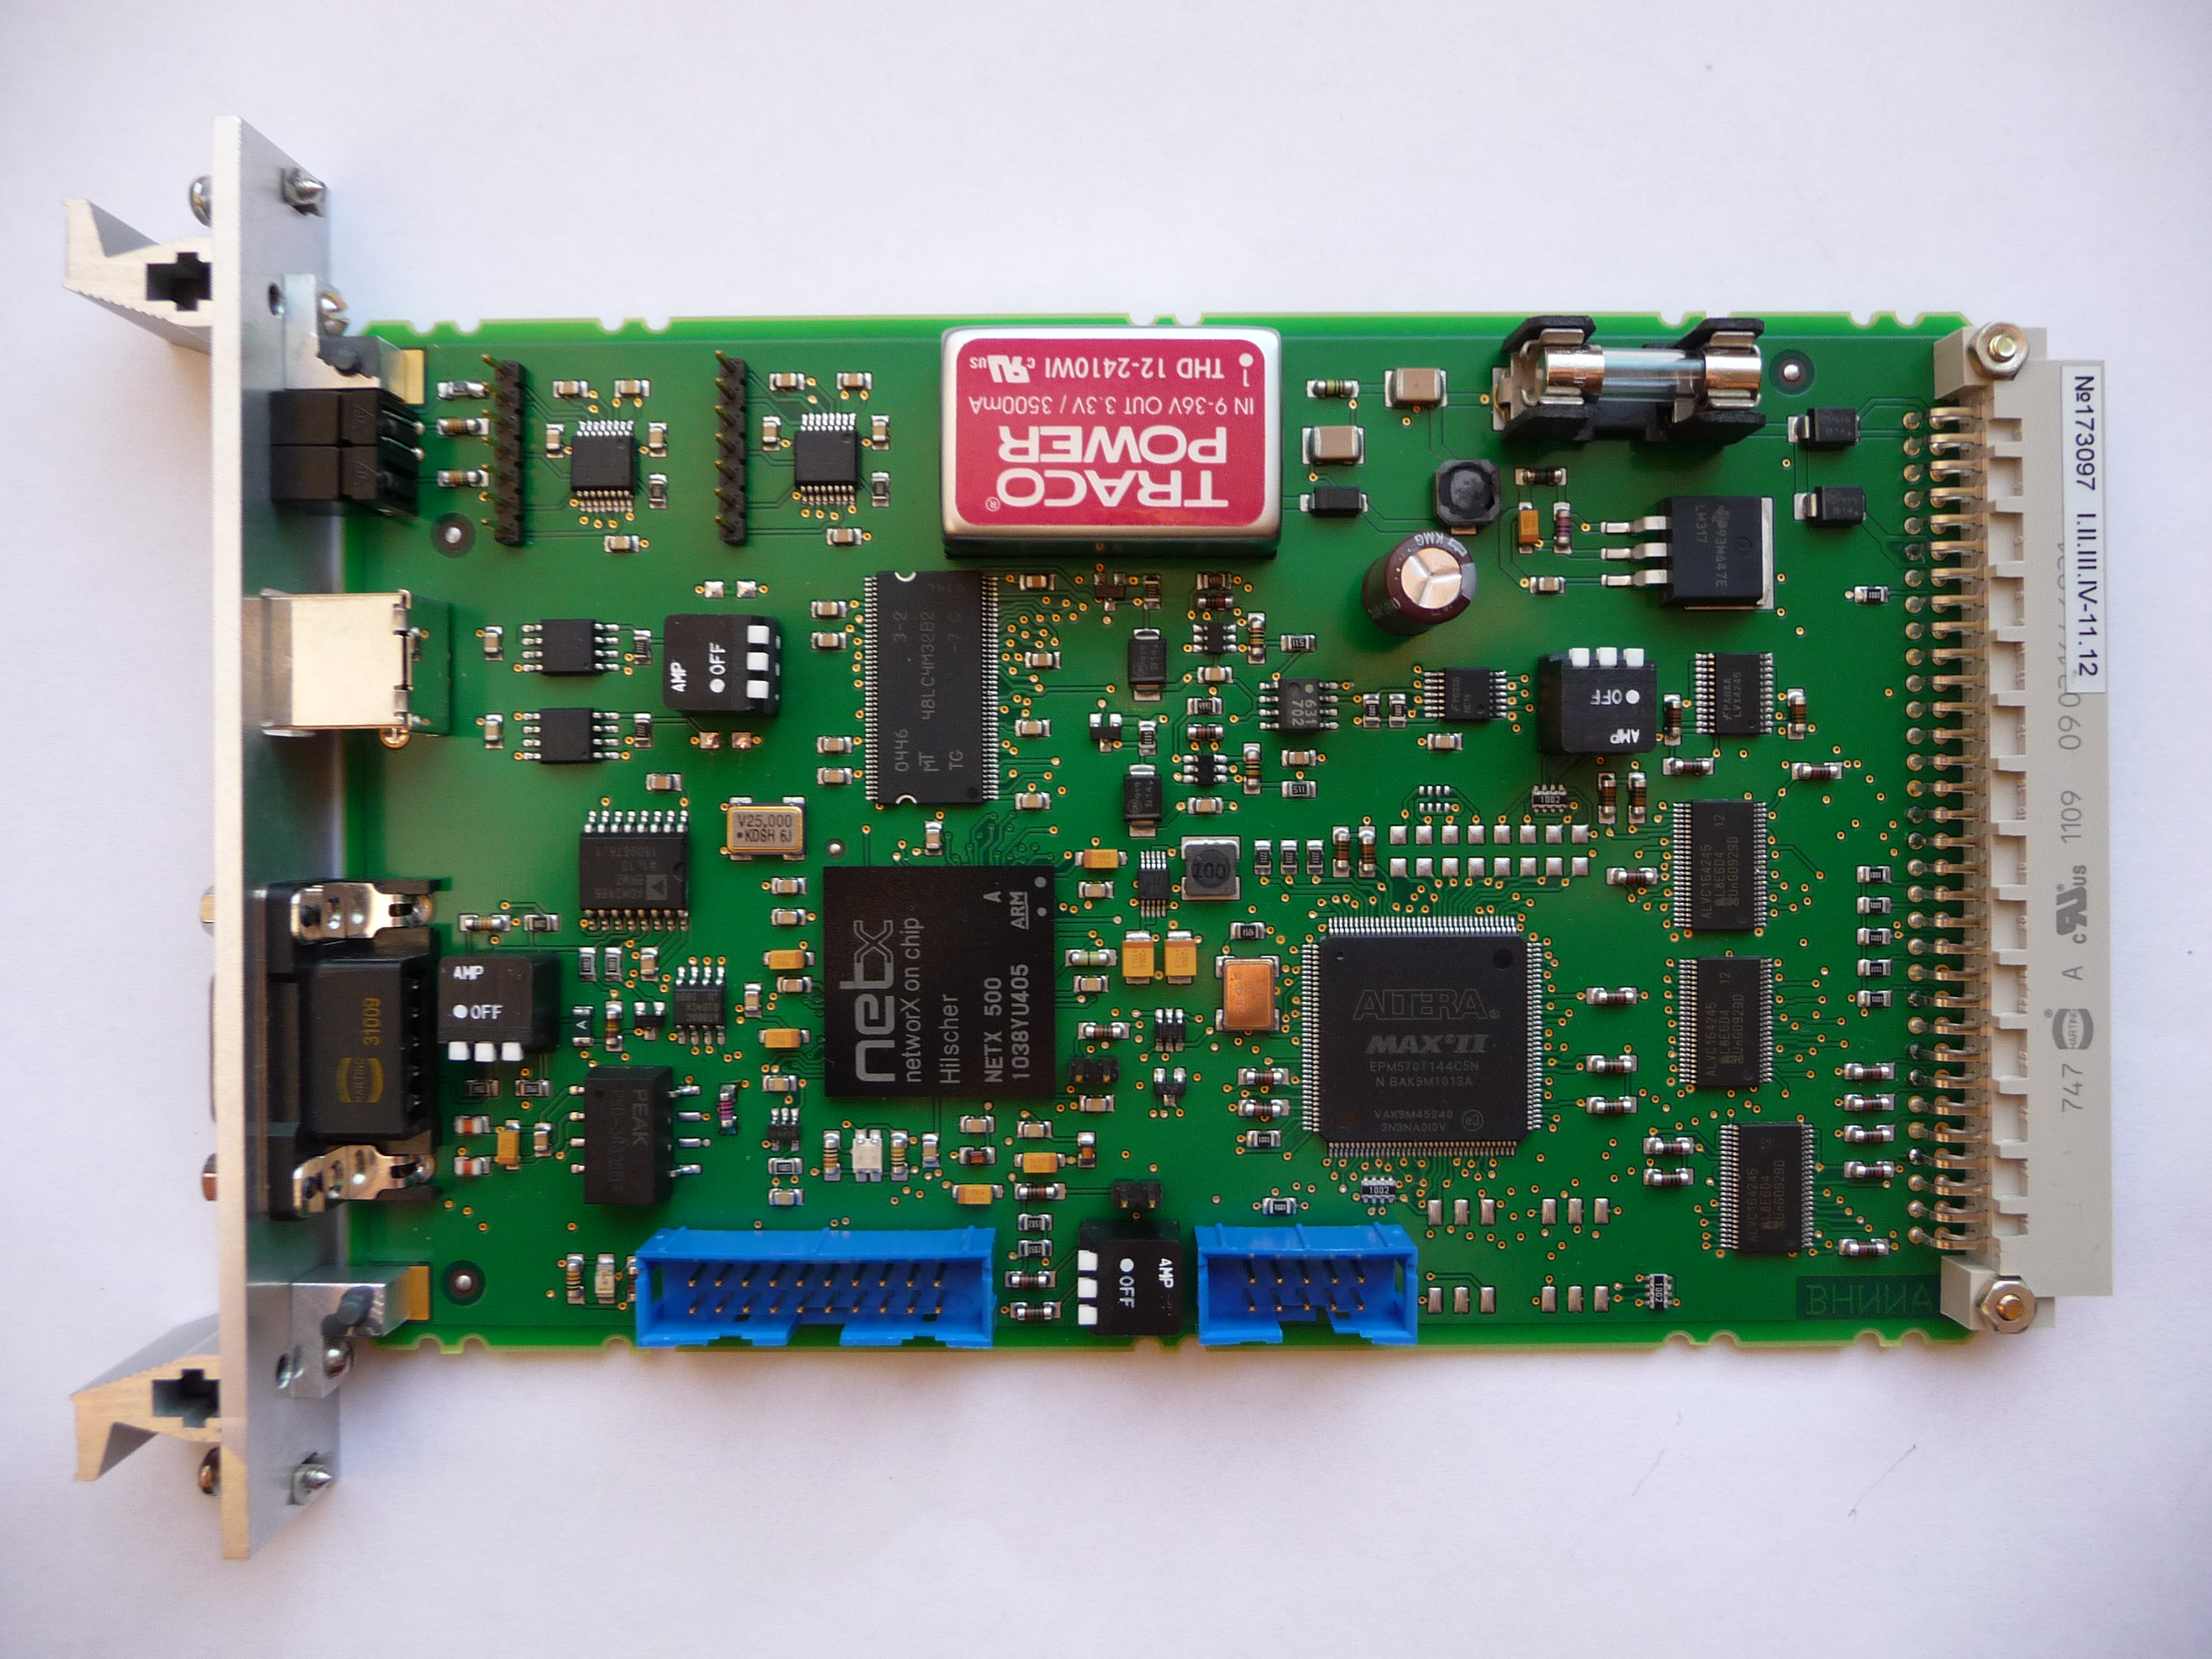
\includegraphics[width=0.9\textwidth]{tpts_1205}
 \caption{\label{tpts_1205} Процессорный модуль ТПТС55.1205}
 \end{center}
\end{figure}

\begin{figure}[H] % вставляем рисунок.
 \begin{center}
 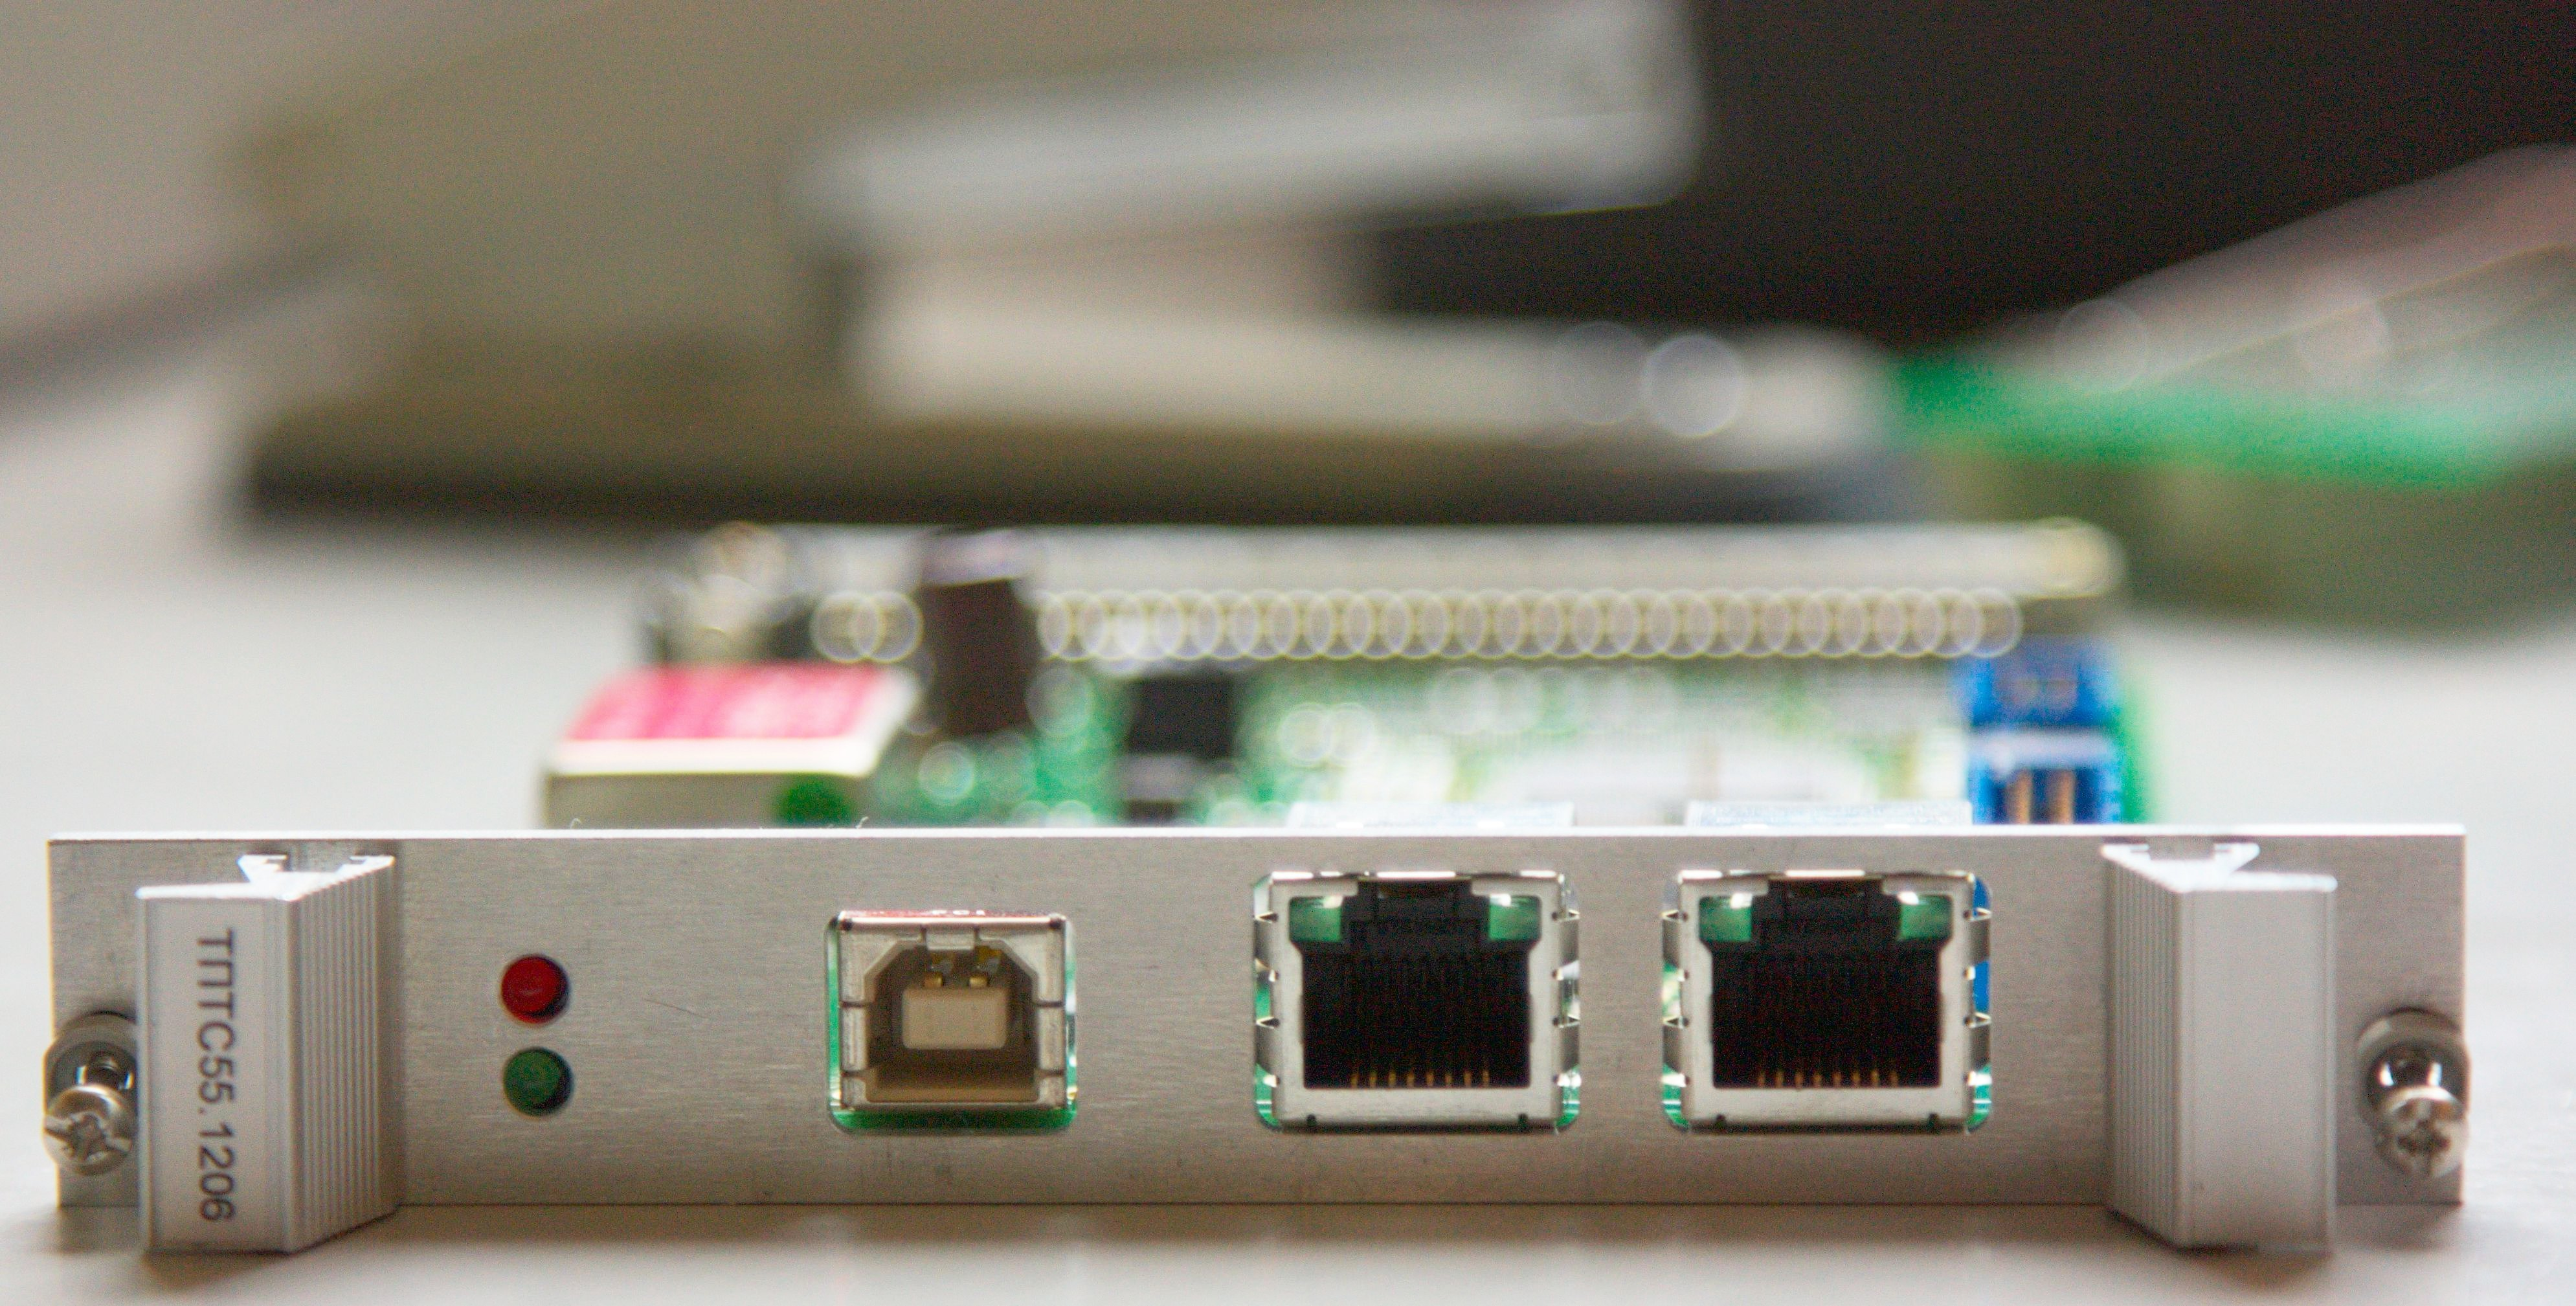
\includegraphics[width=0.9\textwidth]{tpts_1206}
 \caption{\label{tpts_1206} Лицевая панель модуля ТПТС55.1206}
 \end{center}
\end{figure}


Для связи с другими процессорными модулями сервера автоматизации, используется специализированная внутренняя шина связи (ВШС). Реализация протокола обмена происходит при помощи ПЛИС Altera MaxII. Взаимодействие между процессором NetX~500 и ПЛИС осуществляется с помощью SPI-интерфейса, сделанного на основе GPIO, а также при помощи DPRAM процессора. По SPI происходит передача текущего состояния системы, а через DPRAM передаются данные, которые можно считывать по шине ВШС.

Оперативная память реализована на базе микросхемы Micron MT48LC4M32B2-7. Она способна работать на частотах вплоть до 143МГц, рабочая температура данных микросхем составляет -40--85$^\circ$C, то есть полностью идентична таковому у процессора NetX~500.

\chapter{Тестовое программное обеспечения процессорных модулей МС-ПБ}
В процессе выполнения дипломной работы были разработаны две stand-alone программы:
\begin{itemize}
 \item POST -- предназначена для проведения коротких диагностических тестов перед каждым штатным запуском. Главной целью POST-тестов является проверка базовой функциональности процессорного модуля на предмет сбоев.
 \item MT -- предназначена для проведения производственного тестирования (Manufacturing tests), которые служат для диагностики процессорных модулей, в работе которых были зафиксированы ошибки, а также для контроля качества плат, приходящих из производства.
\end{itemize}

\section{Общие архитектурные решения}
В процессе анализа технического задания был принят ряд общих архитектурных решений, влияющих на реализацию как POST, так и производственных тестов:
\begin{itemize}
 \item Каждая плата содержит обе системы тестирования.
 \item В случае обнаружения ошибки на этапе POST-тестирования, загрузка встроенного программного обеспечения прерывается. Процессорный модуль переводится в специальный диагностический режим. Во время очередного опроса, сервер автоматизации читает содержимое регистра PREG микросхемы ПЛИС, в котором содержится информация о текущем состоянии модуля.
 \item Каждая из тестовых программ располагается в своей микросхеме памяти SPI Flash. Выбор микросхемы осуществляется аппаратно, при помощи соответствующей перемычки. Тесты POST не выполняются при запуске MT-тестов, так как это противоречит идеологии производственного тестирования -- производственные тесты служат для детальной диагностики системы в случаи поломки или после поступления плат с производства, поэтому прерывать загрузку тестового программного обеспечения недопустимо ни при каких обстоятельствах.
 \item Предусмотрена возможность использования нескольких образов программного обеспечения, записанных последовательно в память. Несколько образов объединяются в один файл, который записывается в SPI Flash. Каждый образ имеет заголовок определенного формата (NetX Bootblock), содержащий информацию о размере образа и его контрольную сумму. Таким образом, можно простым поиском соответствующих заголовков определить начало и конец необходимой программы и загрузить её. Загрузчик первого уровня всегда загружает только первую программу.
 \item Для упрощения сборки, на ряду со встроенной в HiTOP системой сборки, применяется вторая система на базе Make\cite{make}. Это позволяет с помощью одной команды собрать готовый для использования образ со всем необходимым программным обеспечением, тогда как встроенная система сборки HiTOP не позволяет получить полностью готовый образ.
\end{itemize}

Более подробно каждый тип тестов описывается далее в соответствующих разделах.

Вся информация, необходимая для реализации конкретных тестов, находится в документации на процессор\cite{tech_ref} и в руководстве разработчика\cite{program_ref}. 

\section{Алгоритмы тестирования}
\subsection{Тест SDRAM}
Данный тест обеспечивает проверку шин адреса/данных, а также комплексную проверку памяти SDRAM процессорного модуля. Тест должен выполняться после инициализации внешней SDRAM\cite{optimize}.

Проверяется наличие коротких замыканий или обрывов линий шины данных SDRAM, для чего в SDRAM записываются тестовые последовательности вида:
\begin{center}
\begin{longtable}{c}
\texttt{0xAAAAAAAA}\\
\texttt{0xCCCCCCCC}\\
\texttt{0xF0F0F0F0}\\
\texttt{0xFFFFFFFF}\\
\texttt{0x88888888}\\
\texttt{0x00000000}\\
\end{longtable}
\end{center}
задающие противоположные состояния (0/1) для всех битовых пар (любой пары линий шины данных); всего таких последовательностей получается шесть (для любой пары бит какая-то из последовательностей задаёт противоположные состояния в этой паре, следовательно, независимо от разводки проверяются все "соседние" линии, поэтому в случае замыкания одной линии на другую - в соответствующей последовательности при чтении получим не противоположные состояния, а одинаковые (нулевые)):
\begin{center}
\begin{longtable}{c}
\texttt{0xAAAAAAAAAAAAAAAA}\\
\texttt{0xCCCCCCCCCCCCCCCC}\\
\texttt{0xF0F0F0F0F0F0F0F0}\\
\texttt{0xFF00FF00FF00FF00}\\
\texttt{0xFFFF0000FFFF0000}\\
\texttt{0xFFFFFFFF00000000}\\
\end{longtable}
\end{center}

Для проверки коротких замыканий (КЗ) линий шины данных на другие сигналы (например, если D0 имеет КЗ на землю - с помощью перечисленных выше последовательностей это не будет обнаружено, т.к. во всех них используется 0 в нулевом бите) - тест дополняется ещё шестью последовательностями, инверсными относительно перечисленных выше:
\begin{center}
\begin{longtable}{c}
\texttt{0x0000FFFF}\\
\texttt{0x00FF00FF}\\
\texttt{0x0F0F0F0F}\\
\texttt{0x33333333}\\
\texttt{0x55555555}\\
\end{longtable}
\end{center}

Для обнаружения неподключенных линий шины данных (floating) после записи каждой из перечисленных выше последовательностей, перед его чтением, в другую ячейку памяти выполняется запись отличного от записанной последовательности, например, \texttt{0x0123456789ABCDEF}.

Наличие КЗ/обрывов адресных линий проявляется в "маппировании" двух различных адресов (отличающихся в одном бите) в одну и ту же физическую ячейку; таким образом изменение данных по одному адресу будет приводить к такому же "изменению" данных по другому адресу.

Для выявления такого рода ошибок выполняется последовательная запись в адреса, отличающиеся в одном бите от базового адреса, проинвертированного содержимого ячейки по базовому адресу с последующей проверкой на предмет изменения после записи содержимого базового адреса:
\begin{center}
\begin{longtable}{l}
	\texttt{0b0000} -- базовый адрес, содержит 0x0\\
	\texttt{0b0001} -- проверяется A0, пишем 0xF (~0x0)\\
	\texttt{0b0010} -- проверяется A1, пишем 0xF (~0x0)\\
	\texttt{0b0100} -- проверяется A2, пишем 0xF (~0x0)\\
	\texttt{0b1000} -- проверяется A3, пишем 0xF (~0x0)\\
	\multicolumn{1}{c}{...}\\
\end{longtable}
\end{center}

Например, если имеется обрыв A1, то после выполнения соответствующего теста по базовому адресу будет обнаружено 0xF.

Также, для выявления остальных случаев отказа памяти (перегрев, брак, проявляющийся под нагрузкой), выполняется последовательное заполнение различными последовательностями различных областей SDRAM. Сами последовательности задаются специальным параметром теста.

В случае ошибок будет выведена следующая информация:\\
\verb|ram_test#: 0xADDR bad pattern 0xREAD (expect 0xPATTERN)|, где \# - номер теста; ADDR -- адрес, при проверке которого была обнаружена ошибка; READ -- значение, которое было прочитано; PATTERN -- значение, которое ожидалось.

\subsection{Тест EPROM}
Данный тетст обеспечивает проверку внешней последовательной энергонезависимой перепрограммируемой памяти SPI Flash.

Тест выполняет считывание и расчет контрольной суммы содержимого SPI Flash памяти. Алгоритм расчета контрольной суммы можно представить по формуле: $$SUM=-\sum_0^{max}DWORD$$

То есть происходит знаковое суммирование (с переполнением) всех слов (4 байта) и домножение результата на -1. Данный алгоритм используется потому, что запись такой контрольной суммы осуществляет программа Bootwizard на этапе создания образов бинарных файлов. Дополнительно, аналогичной контрольной суммой защищается сам bootblock каждого из имеющихся образов прошивок.

\subsection{Тест FPGA}
Данный тест обеспечивает проверку связи с ПЛИС, реализующей интерфейс к шине ВШС. Проверка связи с ПЛИС осуществляется по интерфейсу SPI, используемому для передачи результатов тестирования в ПЛИС. В случае POST-тестирования, данный тест повторно записывает текущее состояние POST (регистр PREG) и проверяет, что полученное из ПЛИС в результате этой записи содержимое регистра PREG инверсно отправленному. В случае производственного тестирования, выполняется запись не текущего состояния POST-тестов, а специальной последовательности \texttt{0xDEADBEEF}.

\subsection{Тест LED}
Осуществляется включение всех имеющихся светодиодов на плате на определенные промежутки времени.

\subsection{Ethernet}
Ethernet реализуется через программируемый контроллер xC процессора NetX500. Содержатся три подтеста:
\begin{enumerate}
 \item eth\_raw -- тестирование при помощи компьютера. Обмен LLC-датаграммами, проверка отправленных и полученных результатов
 \item eth\_loop -- проверка без участия ПК. Оба разъема Ethernet платы соединяются кросс-кабелем и обмен данными происходит в автоматическом режиме
 \item eth\_stat -- отображение статистики за время работы Ethernet контроллера.
\end{enumerate}

Особенностью работы контроллера xC в данном режиме является необходимость использования специального FIFO, называемого PTR\_FIFO. Этот механизм позволяет осуществлять полностью <<прозрачную>> передачу данных из Rx/Tx буфера контроллера Ethernet во внутреннюю память процессора.

\subsection{USB}
Встроенный USB контроллер NetX500, с помощью драйвера входящего в состав ВПО MTCore, программируется на реализацию функций CDC, таким образом, при подключении к ПК плата представляется как USB-CDC устройство. С точки зрения операционной системы ПК, такое устройство функционирует как COM-порт.

На получаемые по USB от ПК данные, тест отправляет эхо-ответ. Для этого, usb-соединение постоянно опрашивается на предмет новых данных.

\subsection{RS485}
RS-485 реализуется через специальный программируемый контроллер xC процессора NetX500. В процессе тестирования оператор посылает некоторую последовательность байт плате, плата инвертирует полученные данные и отсылает обратно.

Для работы контроллера xC, в него предварительно нужно загрузить специальный микрокод, регламентирующий его параметры работы.
 Этот код и процедуры его загрузки реализованы во встроенном программном обеспечении системы производственного тестирования.
\section{Встроенное программное обеспечение для производственного тестирования}
При выполнении производственного тестирования (manufacturing tests) используется следующее программное обеспечение:

\begin{itemize}
 \item на персональном компьютере:
   \begin{itemize}
      \item ОС Windows с набором установленных драйверов коммуникационных интерфейсов, а также вспомогательных библиотек (например, WinPCAP для работы с сетевыми картами);
      \item WinMT - разработанная в рамках данного проекта программа производственного тестирования для ПК; задача данной программы заключается в управлении процессом тестирования и сборе результатов тестирования;
   \end{itemize}
 \item на вспомогательном процессорном модуле EN-C ТПТС-НТ:
   \begin{itemize} 
      \item специализированное, модифицированное для данного проекта, встроенное программное обеспечение (ВПО) процессорного модуля EN-C. В качестве базы используется стандартное ВПО данного процессорного модуля (разработанное каф. 27 в рамках предыдущих работ с ВНИИА). Стандартное ВПО модуля содержит реализацию протокола RMAP (Remote Module Access Protocol), с помощью которого обеспечивается опосредованный, через EN-C, обмен ПК (WinMT) с тестируемым процессорным модулем ТПТС55.1205 или ТПТС55.1206. Отличие специализированного ВПО от стандартного заключается в экспортировании через MEMORY группу функций RMAP дополнительных областей адресного пространства EN-C, соответствующих Register и DPRAM областям МС-ПБ на шине ВШС (в стандартном ВПО в MEMORY экспортируются только SDRAM и Flash самого, EN-C, модуля; здесь же эти области дополнены областями ICB\_REG и ICB\_DP, обращения к которым автоматически транслируются в соответствующие обращения к процессорному модулю по шине ВШС).
    \end{itemize}

 \item на тестируемых процессорных модулях комплекса ТПТС-НТ:
  \begin{itemize}
     \item встроенное программное обеспечение (ВПО) MT, разработанное в рамках данного проекта.
  \end{itemize}
\end{itemize}

ВПО MT состоит следующих основных программных модулей:
\begin{itemize}
 \item MTCore: программный модуль, запускаемый загрузчиком первого уровня процессора netX; обеспечивает проверку оборудования с использованием интерфейсов низкого уровня (регистровый доступ к ресурсам netX500: тестирование CPU, SDRAM, ...);
\end{itemize}

MTCore представляет собой программу (один проект в HiTOP), запускаемую во внутренней SRAM контроллера загрузчиком первого уровня процессора netX. Для реализации части тестов необходимо использование ОЗУ, поэтому MTCore представляет из себя два исполняемых файла, компилируемых с поддержкой различных групп тестов:
\begin{enumerate}
 \item Тесты, при своем исполнении не использующие SDRAM: тест sdram, тест EPROM, тест USB.
 \item Тесты, требующие для своей работы SDRAM: тест Ethernet, тест Profibus, тесты ПЛИС и остальные
\end{enumerate}

Для реализации тестов ethernet, usb и profibus необходимо выделение памяти под различные буферы, например для Ethernet необходим буфер размером более 100КБайт. Всего оперативной SRAM памяти доступно 144КБ, поэтому разместить все тестовые функции в ней не представляется возможным. Для решения данной проблемы было принято решение разделения MTCore на две части. Передача параметров между приложениями осуществляется через специальный буфер во внутренней SRAM-памяти процессора, так как данная память не обнуляется при программной переинициализации процессора.

Также следует отметить, что представляется целесообразным не выполнять POST-тестирование перед запуском программы MT. Поскольку при производственном тестировании требуется реализовать возможность выполнения большей части тестов из POST (с отличными от используемых в POST параметрами), то практически все тесты POST-программы присутствуют в программе MT.

Программное обеспечение MT устанавливается в вспомогательную SPI Flash-2 микросхему процессорного модуля. Для установки ПО MT, а также для последующей его активации, перемычки выбора сигнала chip-select SPI Flash микросхем на процессорном модуле должны быть установлены в положение, подключающее микросхему SPI Flash-2 к выходу CS0 контроллера netX500.

ВПО MTCore после своей загрузки, отправляет статусное сообщение в вспомогательный UART процессорного модуля и ожидает поступления команды на выполнение того или иного теста.

По получению команды выполняется её анализ, извлечение параметров и передача управления в соответствующую тестовую функцию.

После завершения выполнения тестовой функции ВПО отправляет в вспомогательный UART сообщение с информацией о результатах только что выполненного теста.

\subsection{Протокол обмена данными с ПК}
Обмен выполняется по протоколу Manufacturing Test Protocol (MTP), разработанному в рамках данного проекта. Все сообщения протокола MTP представляют собой строки состоящие из символов ASCII из интервала от 0x32 (Space) до 0x7E ('$~$') и символа перевода строки '$\backslash{n}$' (EOL, ASCII код 0x0A), который используется в качестве признака конца сообщения. Все остальные символы - игнорируются.

Поскольку протокол ASCII-based, то для работы может быть использована не только WinMT, но и любая другая терминальная программа (Windows HyperTerminal, kermit, ...). Протокол MTP определяет следующий формат для сообщений:
\begin{itemize}
\item команда запуска теста (от ПК в ПМ):

	\verb|run <test_name> --<pname>=<pval0> ... --<pname>=<pvalN>[EOL]|\\
	где

	\begin{itemize}
		\item \verb|<test_name>|: имя теста (одно из значений в "Имя теста" в таблице \ref{mtp_tests}), который требуется запустить; имя теста не должно содержать пробелов и может состоять только из латинских букв, цифр и символа подчёркивания;
		\item \verb|<pnameI>, <pvalN>|: имя параметра и его значение;
	\end{itemize}

\item сообщение об ошибке во время попытки выполнить запрошенный тест (от ПМ в ПК):

	\verb|err <test_name> <err_code> <err_info>[EOL]|\\
	где
	\begin{itemize}
		\item \verb|<test_name>|: имя теста, при попытке выполнения которого возникла данная ошибка;
		\item \verb|<err_code>| и \verb|<err_info>|: код ошибки и дополнительная информация по ошибке; коды ошибок приведены в Табл. \ref{mtp_err_codes};
	\end{itemize}

\item информация о результате выполнения теста (от ПМ в ПК):
	
	\begin{verbatim}done <test_name> [OK|ER] <info>[EOL]}\end{verbatim}
	где
	\begin{itemize}
		\item \verb|<test_name>|: имя теста (одно из значений в "Имя теста" Табл.\ref{mtp_tests}), выполнение которого завершилось;
		\item \texttt{OK|ER}: общий статус выполнения теста (успешно или нет);
		\item \verb|info|: опциональная дополнительная информация о выполненном тесте;
	\end{itemize}
\item команда инициирующая сброс MT (от ПК в ПМ):

	\verb|rst[EOL]|

\item статусное сообщение, отправляемое при каждом запуске MTCore (от ПМ в ПК):

	\verb|ini[EOL]|

\item сообщения, которыми могут обмениваться ПК и ПМ для проверки связи:

	\verb|ping [EOL] [MSG]|

	\verb|pong [EOL]|

	команда <ping> (от ПК к ПМ) инициирует выдачу ответа <pong> (от ПМ в ПК);

\item дополнительная или отладочная информация произвольного содержания (от ПМ в ПК):

	\verb|dbg <info>[EOL]|
\end{itemize}

\begin{center}
\addtocounter{tbls}{1}
\begin{longtable}{|l|p{8cm}|}
 \caption{\label{mtp_tests}Названия тестов и их параметры}\\\hline
 Имя теста & Краткое описание \\\hline
\endfirsthead
\multicolumn{2}{c}{Продолжение таблицы \thetable}
\endhead
sdram\_abus & Проверка адресной шины SDRAM \\\hline
sdram\_dbus & Проверка шины данных SDRAM \\\hline
sdram\_cells & Проверка ячеек SDRAM -- инициируется проверка с помощью записи-чтения указанной последовательности в укзанные ячейки \\\hline
eprom\_checksum & Проверка SPI Flash памяти с помощью подсчета контрольных сумм \\\hline
fpga\_spi & Проверка функционирования ПЛИС процессорного модуля с помощью обмена по SPI \\\hline
led\_on & Проверка светодиодов \\\hline
rs485\_xfer & Проверка интерфейса RS-485 \\\hline
eth\_raw & Проверка интерфейсов Ethernet на уровне ethernet-кадров при помощи ПК \\\hline
eth\_loop & Проверка интерфейсов Ethernet на уровне ethernet-кадров в режиме замыкания \\\hline
usb\_com & Проверка интерфейса USB \\\hline
icb\_init & Выполнение инициализации DPRAM \\\hline
icb\_copy & Выполнение копирования данных в DPRAM \\\hline
\end{longtable}
\end{center}

\begin{center}
\addtocounter{tbls}{1}
\begin{longtable}{|l|l|l|p{6cm}|}
\caption{\label{mtp_err_codes}Коды ошибок}\\
\hlineКод & Имя & Дополнительная информация & Описание \\\hline
\endfirsthead
\multicolumn{4}{c}{Продолжение таблицы \thetable}
\endhead
-1 & BAD\_TEST & - & Тест с именем \verb|<test_name>| отсутствует в ВПО MT \\\hline
-2 & BAD\_PNAME & \verb|<pname>| & Тест \verb|<test_name>| не имеет конфигурационного параметра с именем \verb|<pname>|, указанным в команде 'run' \\\hline
-3 & BAD\_PVAL & \verb|<pname>| \verb|<prange>| & Параметр с именем \verb|<pname>| не может принимать заданное в команде значение; указываются также допустимые значения для данного параметра \\\hline
\end{longtable}
\end{center}

\section{Встроенное программное обеспечение POST}
Тесты POST запускаются загрузчиком первого уровня (The 1st Stage Boot\-strap) процессора NetX~500. При этом образ, содержащий программу POST загружается из последовательной памяти (SPI Flash) во внутреннюю RAM процессора. Исполнение кода непосредственно из последовательной памяти не поддерживается процессором.

После выполнения тестовых процедур программа POST загружает из последовательной памяти образ основной программы (программы нормальной эксплуатации) во внешнюю оперативную память процессорного модуля и передает управление ей. Для определения параметров основной программы используются поля структуры netX Bootblock, предваряющие образ программы. Содержимое структуры NetX Bootblock представлено в таблице \ref{bootblock}

\begin{center}
\addtocounter{tbls}{1}
\begin{longtable}{|c|p{10cm}|}
  \caption{\label{bootblock}Структура загрузочного блока} \\\hline
  \endfirsthead
  \multicolumn{2}{c}{Продолжение таблицы \thetable}
  \endhead
  Поле & комментарий \\\hline
  ulMagCok & Определяет тип прошивки: параллельная или последовательная постоянная память \\\hline
  unCtrl & Содержит настройки, необходимые для инициализации микросхемы постоянной памяти \\\hline
  ulAppEnt & Указатель на адрес точки входа в основную программу \\\hline
  ulAppChksum & Контрольная сумма прошивки, представляет из себя побитовый XOR всего ВПО, за вычетом загрузочного блока\\\hline
  ulAppFilSiz & Размер ВПО, в блоках по 4 байта \\\hline
  ulAppSrtAdd & Адрес региона памяти, в который будет загружаться ВПО\\\hline
  ulSignt & Число, всегда равное 0x5854454E (соответствует ASCII представлению слова NETX) \\\hline
  unCtrl0-4 & В зависимости от типа сборки, содержит настройки SDRAM или DPM контроллеров\\\hline
  ulMiscAsicCtrl & Значение внутреннего регистра ASIC (всегда 1) \\\hline
  ulSerial & Серийный номер\\\hline
  ulBootChksum & Контрольная сумма загрузочного блока, вычисляемая как сумма всех блоков по 4 байта, умноженная на -1 \\\hline
\end{longtable}
\end{center}


\subsection{Особенности POST-тестов по сравнению с производственными}
Большинство POST-тестов представляют из себя упрощенные варианты производственных тестов. Из POST-тестов исключены все тесты, которые во время своей работы могут повлиять на какие-либо внешние устройства: тест RS485, тест Ethernet, тест USB. При этом, были добавлены тесты встроенных SRAM и ROM процессора NetX~500.

\subsubsection{Передача информации о состоянии системы}
Результаты выполнения POST-тестов передаются по интерфейсу SPI в ПЛИС процессорного модуля и, впоследствии, доступны для получения из соответствующего регистра PREG с помощью чтения по шине ВШС сервера автоматизации. Старший бит регистра PREG сбрасывается в ноль после выполнения всех тестов, 0-ой (младший бит) сбрасывается в 0 перед началом выполнения первого теста. Остальные биты зарезервированы под статусы выполнения конкретных тестов. При включении питания ПЛИС инициализирует регистр PREG единицами. Содержимое регистра обновляется после каждого теста.

Интерфейс связи (SPI) с ПЛИС организуется программно с использованием цифровых GPIO микропроцессора NetX. По линии MISO ПЛИС возвращает значение, инверсное содержимому регистра PREG (до начала транзакции). Это используется для тестирования работоспособности ПЛИС.

\subsubsection{Тест SRAM}
Особенностью данного теста является необходимость проверки той же части памяти, из которой в данный момент исполняется программа тестирования. Для этого, используется ряд расширений стандарта c90 под названием gnu90:

\begin{enumerate}
 \item Использование свойств \verb|__attribute__ ((section ...))| -- позволяет на уровне скриптов линковки (пример реализации можно увидеть в приложении \ref{sram-ld}) определить границы конкретной функции.
 \item Использование свойств переменных \verb|asm| -- позволяет заставить компилятор использовать указанные регистры под конкретные переменные.
\end{enumerate}

Таким образом, используя эти расширения можно исключить область памяти, занимаемую функцией тестирования, из самого теста. Код теста на языке Си приведен в приложении \ref{sram-c}.

В качестве проверки корректности утверждений, сделанных выше, была сделана сборка с сохранением промежуточного ассемблерного кода в отдельные файлы. В результате анализа кода функции теста было подтверждено, что все её временные переменные хранятся в регистрах, каких-либо непредусмотренных обращений к SRAM памяти не происходит. Ассемблерный код приведен в приложении \ref{sram-asm}.

\section{Программа управления процессом тестирования -- WinMT}
Программа WinMT, исполняющаяся на ПК, обеспечивает управление процессом тестирования и сбор результатов тестирования.

\subsection{Графический интерфейс}
На Рис.\ref{winmt-1} показан интерфейс программы WinMT.

\begin{figure}[h!] % вставляем рисунок.
\addtocounter{myfigs}{1}
 \begin{center}
 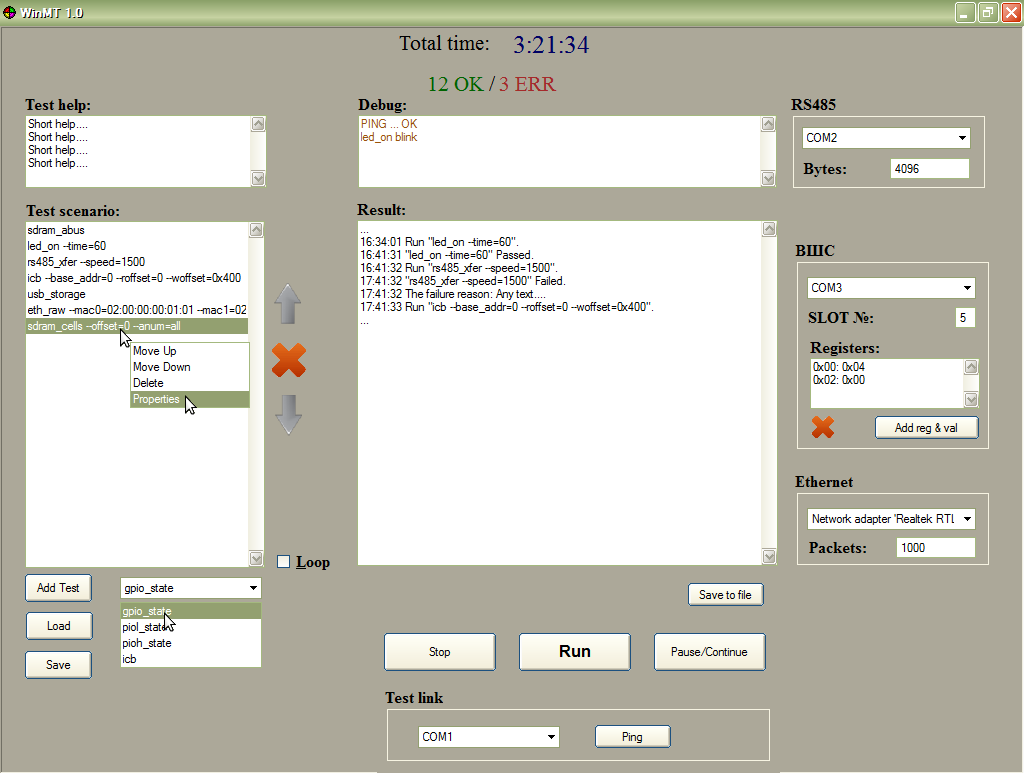
\includegraphics[width=0.9\textwidth]{winmt-1}
 \caption{\label{winmt-1} Основное окно программы WinMT}
 \end{center}
\end{figure}

Окно состоит из следующих областей:
\begin{itemize}
	\item Total time: Полное время от начала запуска тестирования.
	\item OK/ERR: Суммарное количество успешно(OK), и неуспешно(ERR) пройденных тестов.
	\item Test help: Содержит краткую справочную информация о текущем тесте. 
	\item Test scenario: Список тестов, которые будут выполнены при запуске тестирования.
	\item Кнопки изменения порядка тестов и кнопка удаления теста из сценария.
	\item Loop: Флаг "зациклить". Если этот флаг установлен то тестовый сценарий будет выполнятся циклически. То есть после выполнения последнего теста начнёт снова выполнятся первый.
	\item Выпадающий список с выбором нового теста.
	\item Кнопки Save/Load для сохранения текущего сценария в файл, и загрузки из файла предварительно сохранённого сценария (а также параметров RS485, ВШС, Ethernet тестов);
	\item Debug: Окно для вывода дополнительной информации. В основном это информация об ошибках в командах, результат диагностики тестового интерфейса или иная дополнительная информация.
	\item Result: Окно для вывода лога тестирования. В это окно выводится информация о старте тестов, а также результате их прохождения.
	\item Кнопки управления выполнением сценария. Запуск, остановка, пауза/продолжение.
	\item Test link: Область содержит выпадающий список с выбором COM-порта, используемого для подключения тестируемого модуля, и кнопку для диагностики тестового интерфейса (Ping). Результат диагностики тестового интерфейса выводится в окно Debug.
	\item RS485: Область для редактирования параметров теста RS485. Область содержит: выпадающий список для выбора виртуального COM-порта, экспортируемого USB-RS485 контроллером, через который выполняется подключение к RS485 интерфейсу МС-ПБ и поле для ввода количества байт.
	\item ВШС: Область для редактирования параметров теста ВШС. Область содержит: выпадающий список для выбора COM-порта, к которому подключен EN-C и поле для ввода проверяемых через EN-C регистров ВШС МС-ПБ.
	\item Ethernet: Область для редактирования параметров теста Ethernet. Область содержит: выпадающий список для выбора используемой сетевой карты и поле для ввода количества фреймов.
\end{itemize}

На Рис.\ref{winmt-2} показан интерфейс окна редактирования параметров теста. Окно состоит из следующих областей:
\begin{itemize}
	\item Окно, содержащее подробную справочную информация о текущем тесте.
	\item Поле для редактирования параметров теста. (Редактировать можно только параметры теста, имя теста изменять нельзя).
\end{itemize}

\begin{figure}[h!]
\addtocounter{myfigs}{1}
\begin{center}
	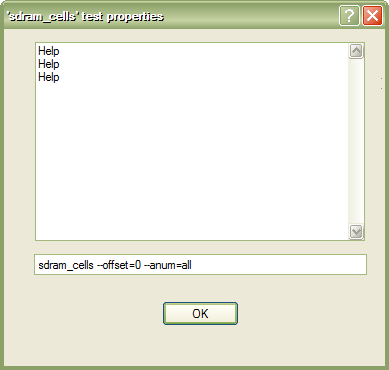
\includegraphics[width=0.4\textwidth]{winmt-2}
	\caption{\label{winmt-2} окно редактирования параметров теста программы WinMT}
\end{center}
\end{figure}

\subsection{Создание тестового сценария}
Тестовый сценарий создаётся путём добавления новых тестов. 

Для добавления нового теста необходимо:
\begin{itemize}
	\item Выбрать имя теста в специальном выпадающем списке. При этом в окне "Test help" отобразится краткая справочная информация о тесте.
	\item Нажать на кнопку "Add Test".
\end{itemize}

Для редактирования параметров теста необходимо:
\begin{itemize}
	\item Выбрать тест в окне "Test scenario".
	\item Вызвать контекстное меню (нажать правой кнопкой мыши на выбранном тесте).
	\item В контекстном меню выбрать пункт "Properties".
	\item Далее в появившемся окне (Рис.\ref{winmt-2}) отредактировать параметры теста.
	\item При создании тестов "RS485", "ВШС", или "Ethernet" необходимо также отредактировать дополнительные параметры, они находятся в соответствующих областях в основном окне программы.
\end{itemize}

Для удаления теста из сценария необходимо:
\begin{itemize}
	\item Выбрать тест в окне "Test scenario".
	\item Нажать на кнопку удалить (иконка в виде крестика справа от окна "Test scenario").
\end{itemize}

Для работы со сценариями можно также пользоваться кнопками Save и Load, которые позволяют сохранить (и впоследствии загрузить) сформированный тестовый сценарий в виде текстового файла на жёстком диске ПК.

Для запуска, созданного тестового сценария, необходимо нажать на кнопку "Run". После запуска программа будет последовательно выполнять все тесты. Результат выполнения тестов отображается в окне "Result".
\section{Результаты тестирования модулей МС-ПБ}
Первая партия плат поступила из производства в конце 2011 года. Все они были протестированы с помощью программы производственного тестирования. Результаты тестирования первых полученных образцов представлены в таблице \ref{test-result}.

\begin{center}
\addtocounter{tbls}{1}
\begin{longtable}{|c|c|c|c|}
\caption{\label{test-result}Результаты прохождения тестов}\\
\hline & ТПТС55.1205 & ТПТС55.1206 & Плата развития \\\hline
\endfirsthead
\multicolumn{4}{c}{Продолжение таблицы \thetable}
\endhead
EPROM & + & + & + \\\hline
Ethernet & + & N/A & + \\\hline
FPGA & - & - & N/A \\\hline
GPIO & + & + & + \\\hline
DPRAM & - & - & N/A \\\hline
LED & + & + & + \\\hline
RS485 & N/A & + & + \\\hline
SDRAM & + & + & + \\\hline
USB & + & + & + \\\hline
\end{longtable}
\end{center}

<<N/A>> обозначает, что на данной плате тест выполнить невозможно из-за аппаратных ограничений -- отсутствие нужных для выполнения тестов компонентов или разъемов. На момент поступления плат из производства было заранее известно, что в них существуют некоторые недоработки -- отсутствует работоспособная программа для ПЛИС (тестируется тестом FPGA), а от работоспособности ПЛИС зависит тест DPRAM, таким образом данное поведение является допустимым и нормальным. К сожалению, из-за присутствующих недостатков плат, не удалось убедиться в работоспособности и корректности тестов DPRAM и FPGA.

Тестовый стенд представлен на рисунке \ref{test-stend}. Также предусмотрен упрощенный вариант тестового стенда, не позволяющий тестировать ВШС, но значительно более компактный. Он представлен на рисунке \ref{stend-alone}

\begin{figure}[H]
\addtocounter{myfigs}{1}
\begin{center}
	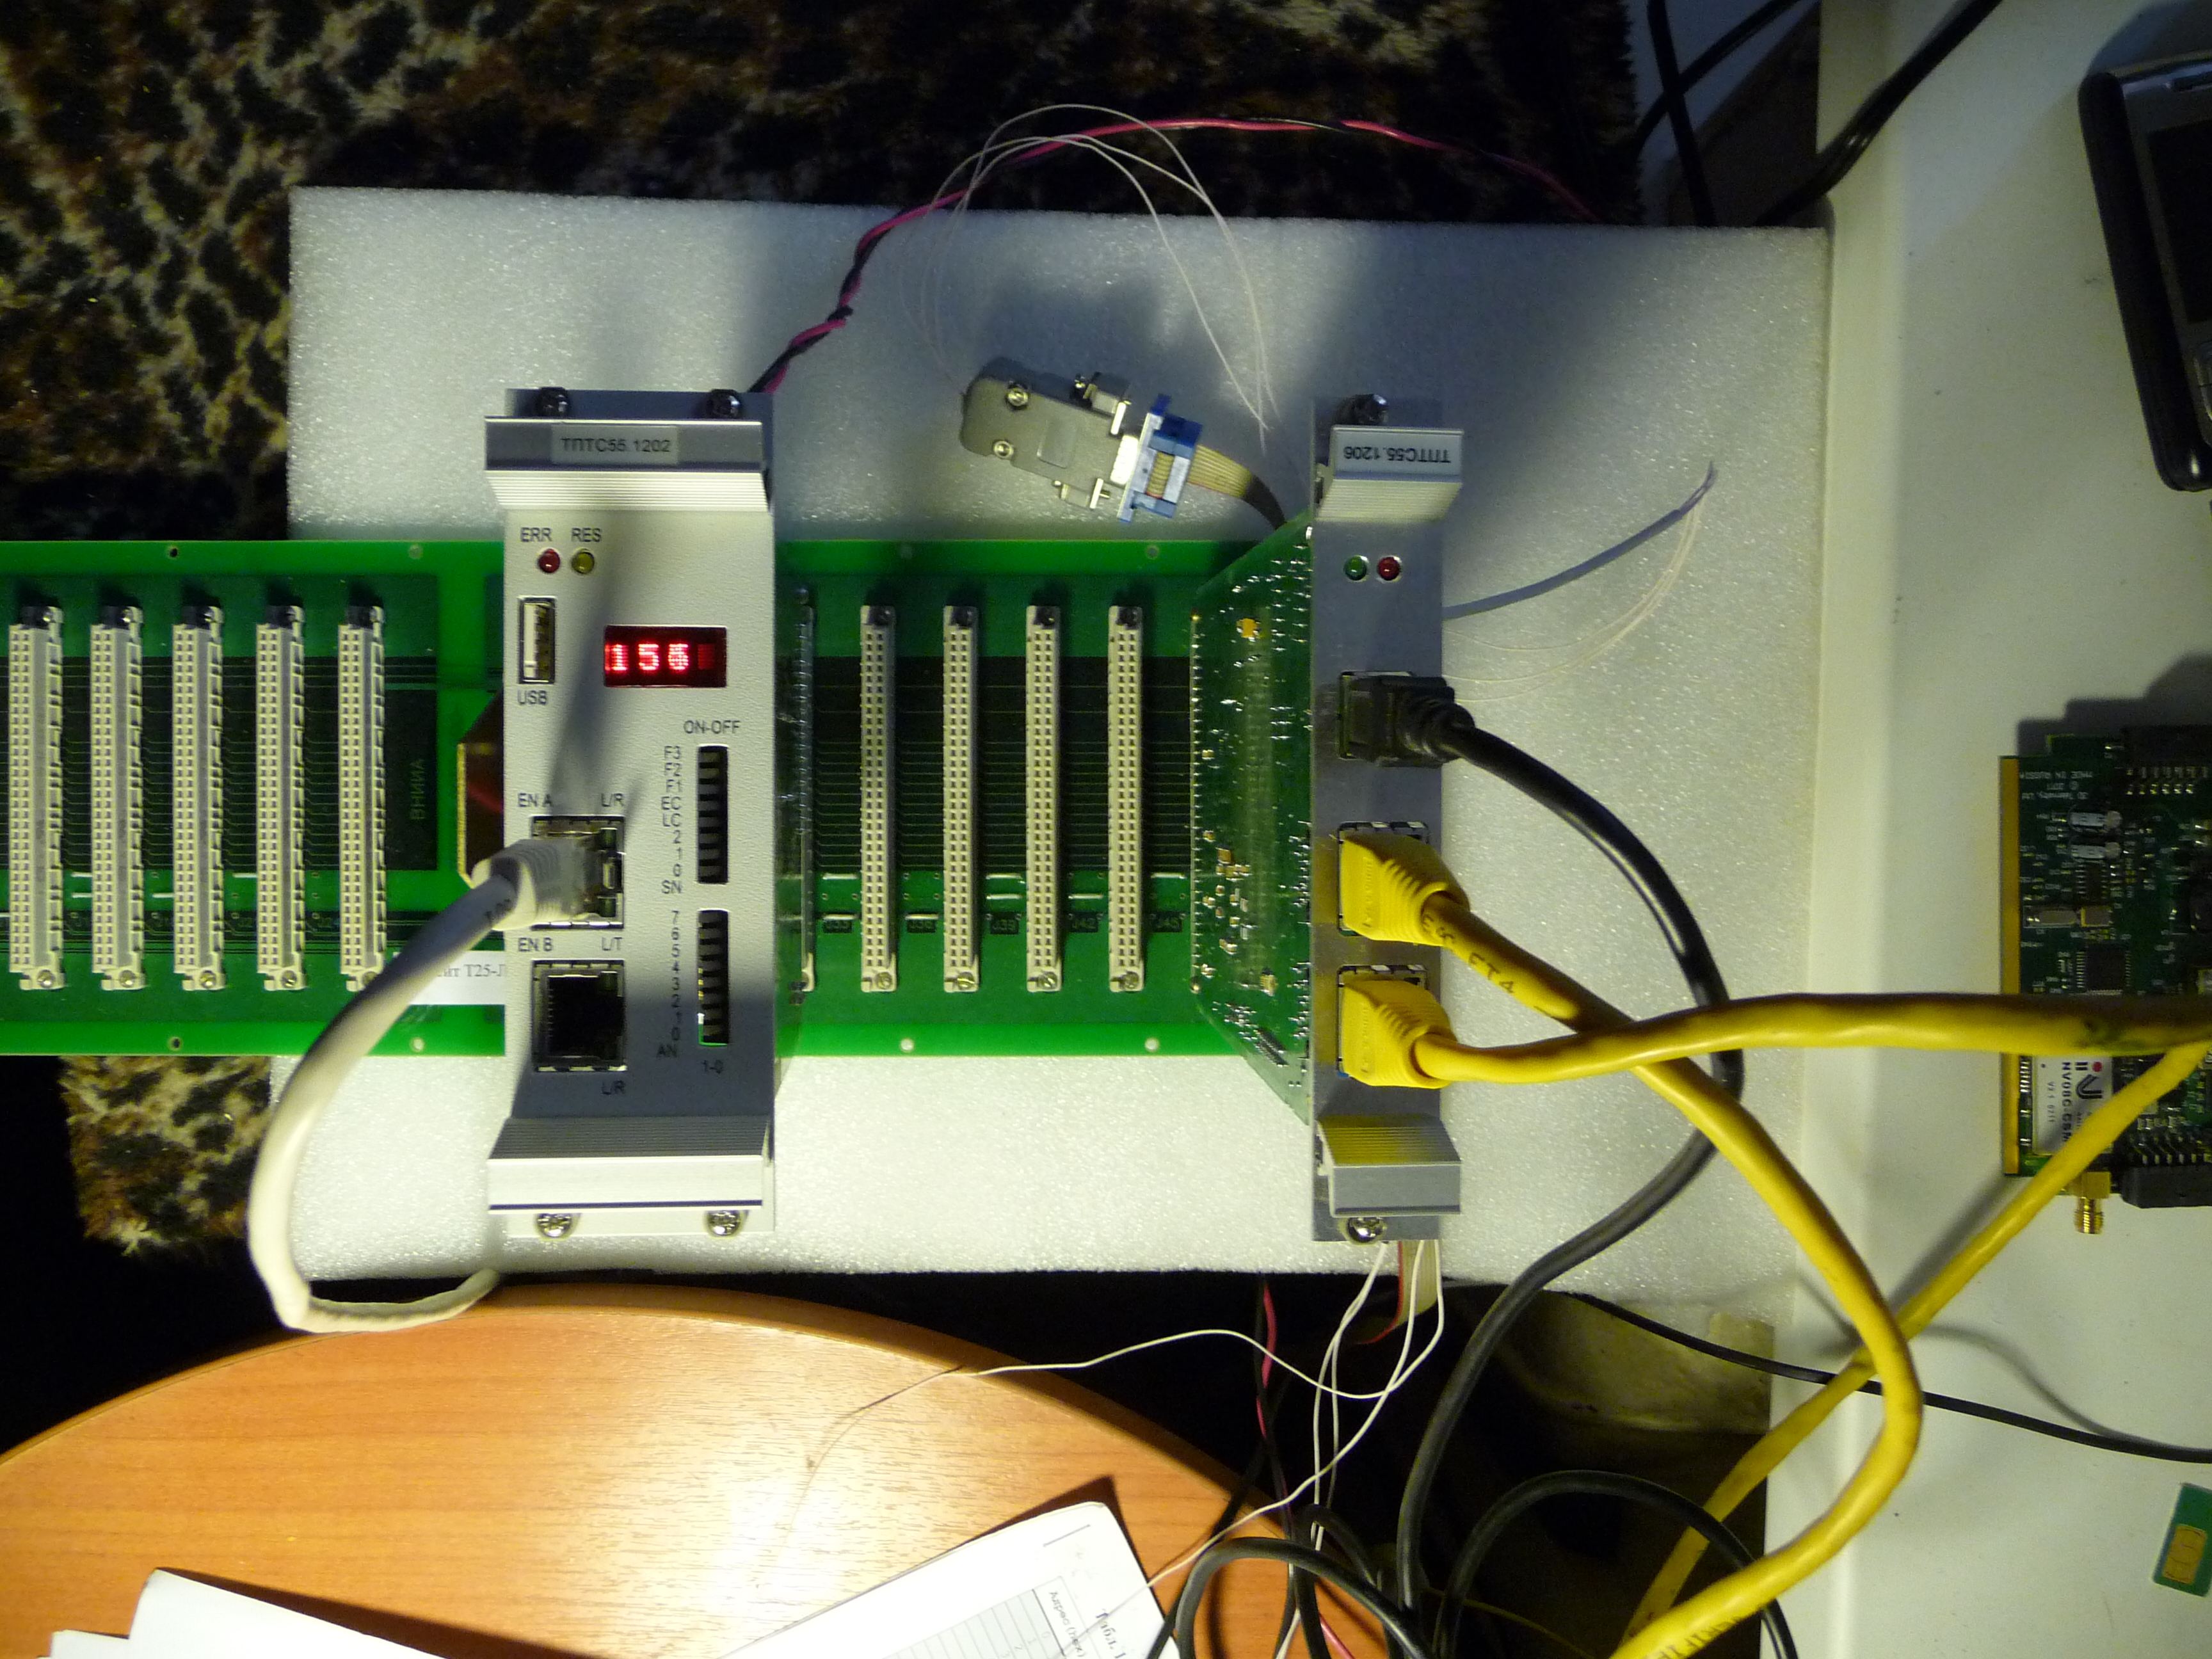
\includegraphics[width=0.8\textwidth]{P1030169}
	\caption{\label{test-stend} Стенд комплексного производственного тестирования}
\end{center}
\end{figure}

\begin{figure}[H]
\addtocounter{myfigs}{1}
\begin{center}
	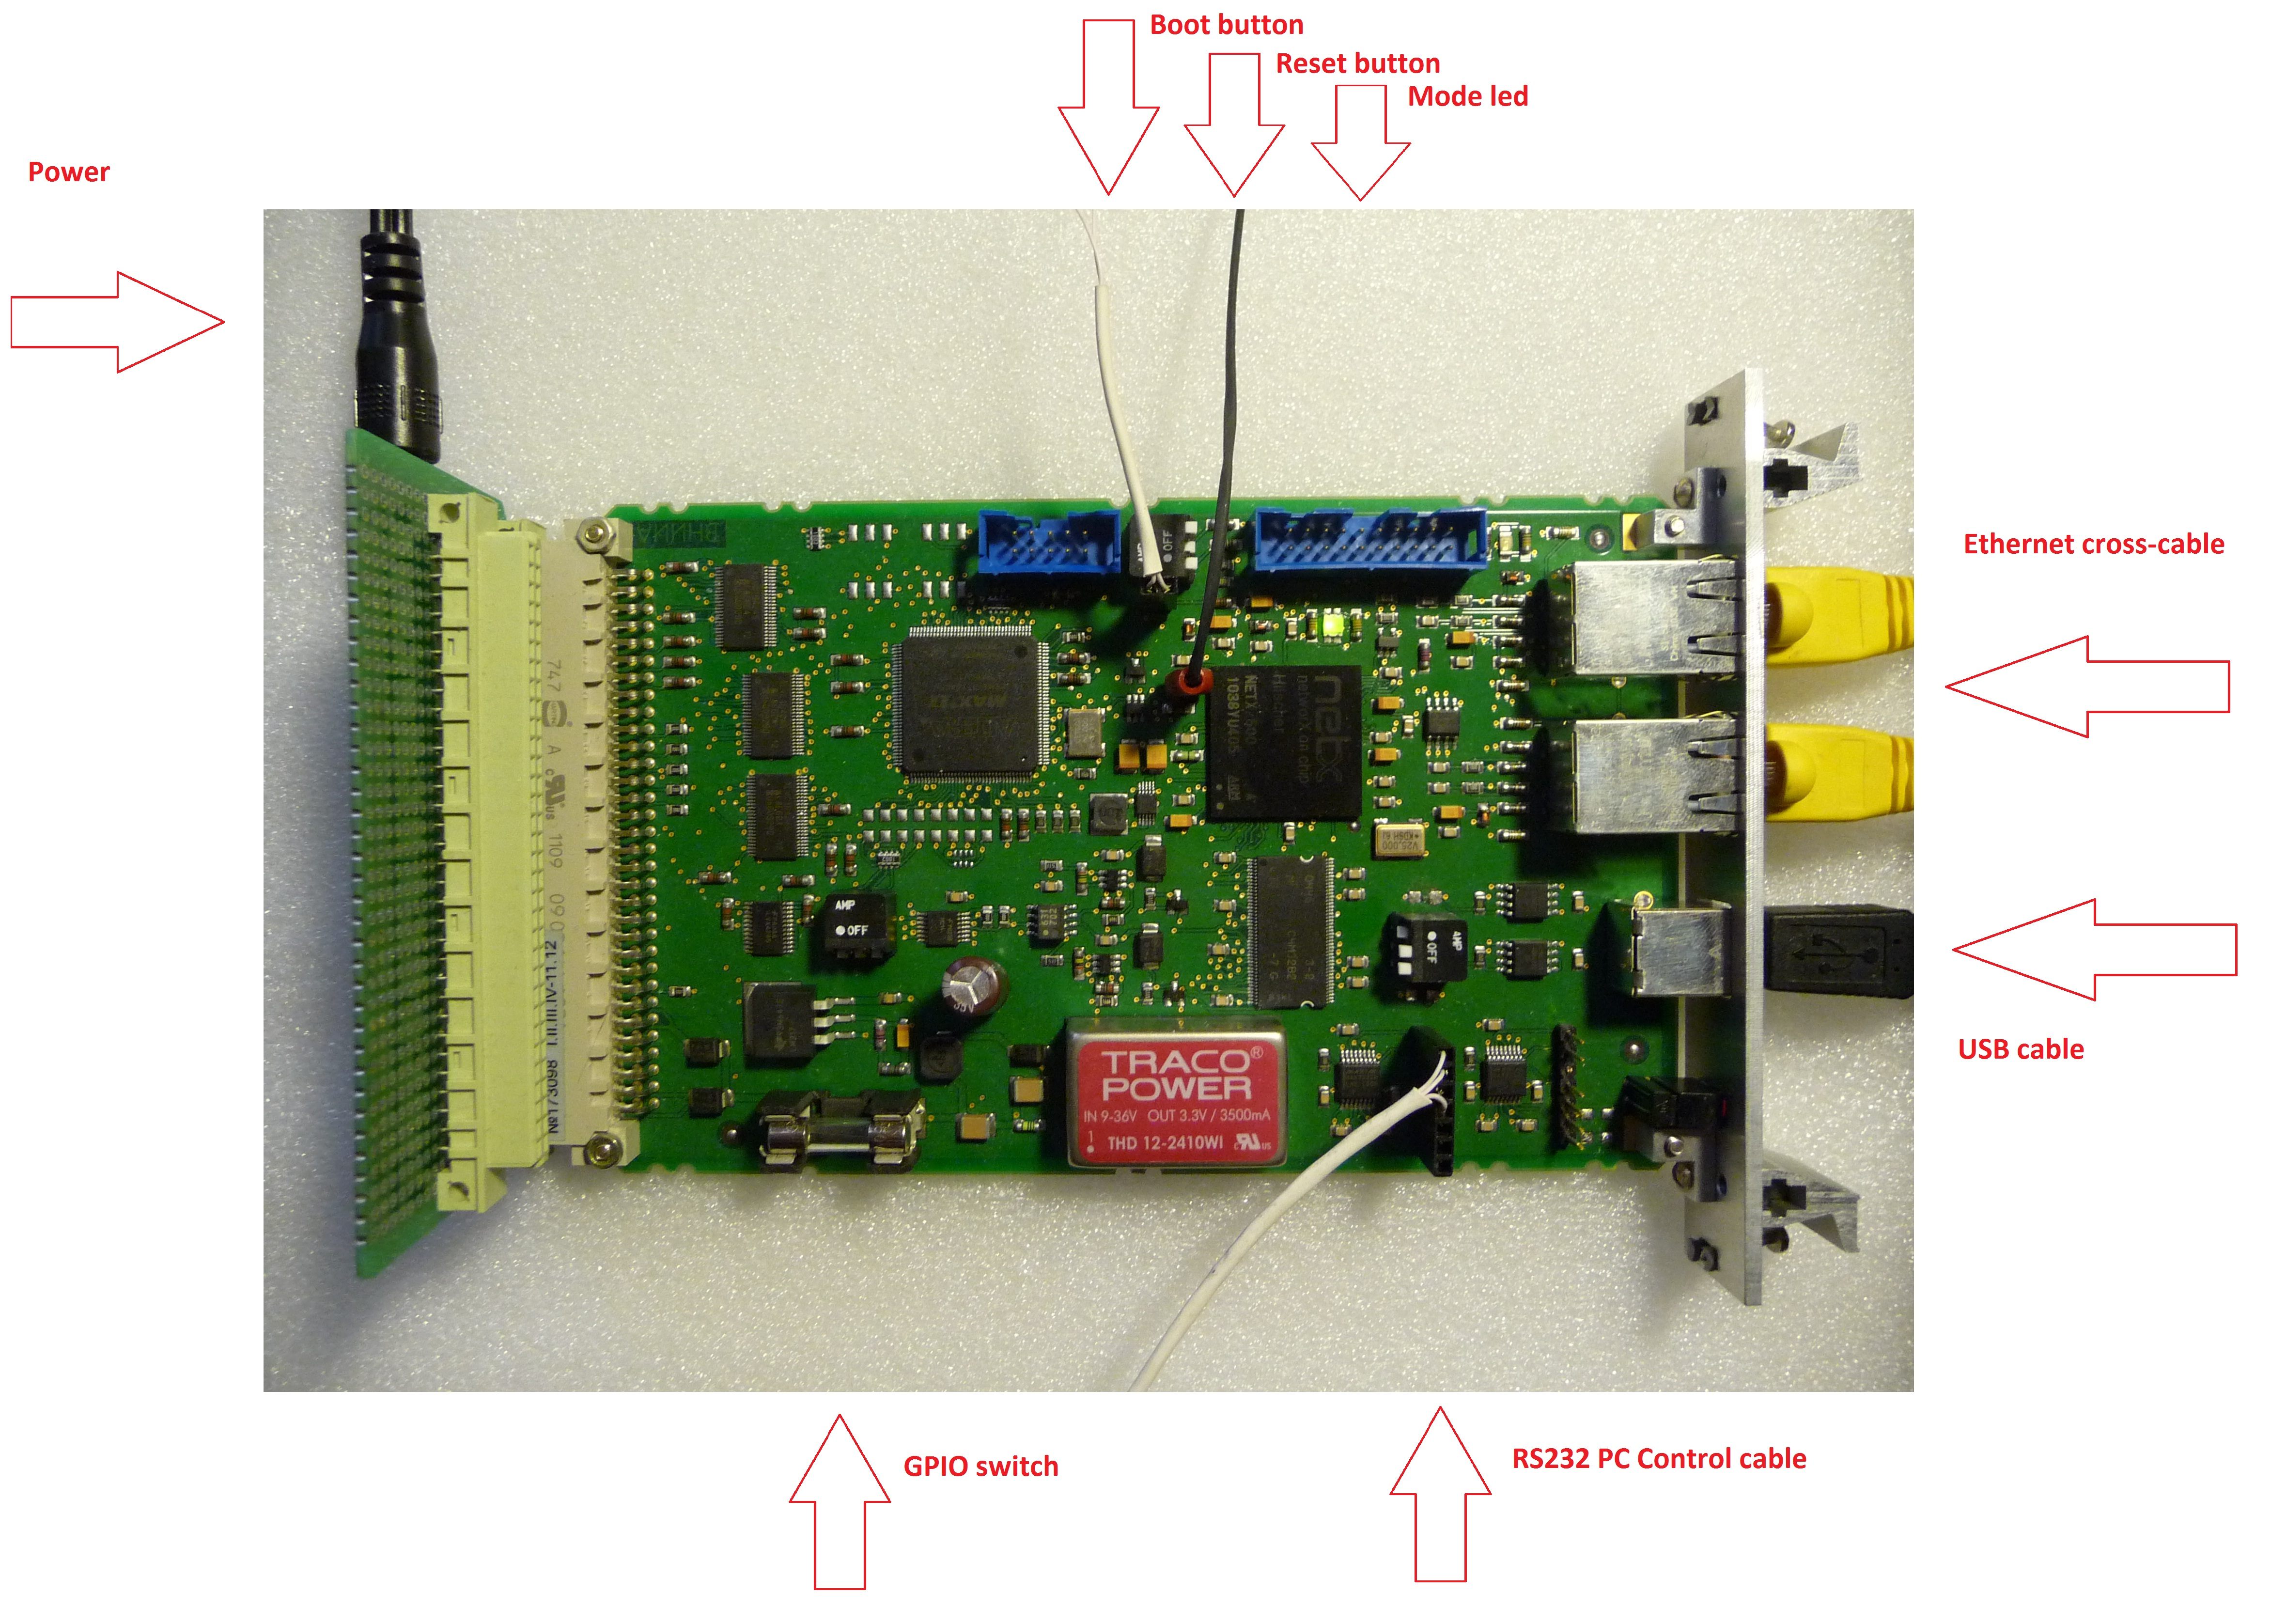
\includegraphics[width=0.8\textwidth]{stand-alone}
	\caption{\label{stend-alone} Упрощенный вариант тестового стенда}
\end{center}
\end{figure}

Пример сценария WinMT приведен в приложении \ref{scr}. Результат работы тествого сценария представлен в приложении \ref{log}. Окно программы WinMT после прохождения теста представлено на рисунке \ref{1206-ok}.

\begin{figure}[H]
\addtocounter{myfigs}{1}
\begin{center}
	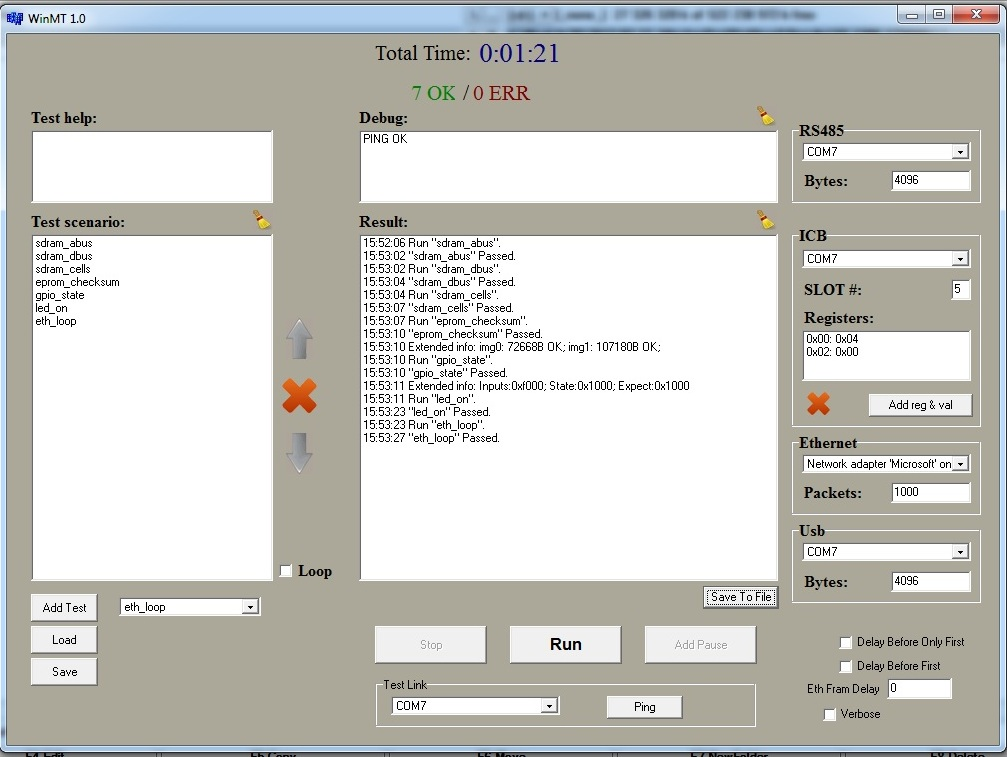
\includegraphics[width=0.8\textwidth]{1206-ok}
	\caption{\label{1206-ok} Результаты прохождения цикла производственного тестирования платой ТПТС55.1206}
\end{center}
\end{figure}


\chapter{Заключение}
В ходе выполнения дипломного проекта велась работа по реализации тестового программного обеспечения для процессорных модулей, выполненных на базе микропроцессоров Hilscher~NetX~500, используемых в составе серверов автоматизации комплексов ТПТС-НТ.

В результате выполнения дипломного проекта:
\begin{itemize}
 \item Разработано встроенное программное обеспечения для проведения оперативных POST тестов.
 \item Разработано встроенное программное обеспечение для проведения производственных тестов.
 \item Разработан протокол взаимодействия ПК со встроенным программным обеспечем для проведения производственных тестов.
 \item Разработана среда управления и автоматизации выполнения тестовых процедур.
\end{itemize}

По результатам дипломного проекта был представлен стендовый доклад на научной сессии \cite{stendMephi}, проходившей в НИЯУ МИФИ в 2012 году.

В данный момент ожидается поступление новой ревизии плат из производства, поставка полноценного тестового стенда со всем необходимым оборудованием, для тестирования DPRAM и Profibus.

\bibliographystyle{utf8gost780u}
\begin{thebibliography}{00} %% здесь библиографический список
\bibitem{rcX} Hilscher Realtime Communictaion System for netX, Kernel API Function Reference
\bibitem{TZ} Разработка аппаратных и программных средств модуля связи комплекса ТПТС-НТ с шиной PROFIBUS-DP
\bibitem{program_ref} Hilscher NetX Program Reference Guide
\bibitem{tech_ref} Hilscher NetX Technical Data Reference Guide

\bibitem{shildt} Г.Шилдт. Полный справочник по C --- Вильямс, 2009.
\bibitem{Sheg} И.И. Шагурин. Современные микроконтроллеры и микропроцессоры --- Горячая Линия -- Телеком, 2004.
\bibitem{Griffits} А.Гриффитс. GCC. Полное руководство --- ТИД <<ДС>>, 2004.
\bibitem{make} Robert Mecklenburg. Managing Projects with GNU Make, 3rd Edition --- O'Reilly Media, 2004.
\bibitem{optimize} К. Касперски. Техника оптимизации программ. Эффективное использование памяти --- BHV, 2003.

\bibitem{stendMephi} Научная сессия НИЯУ МИФИ-2012, Аннотации докладов, стр. 133, Типография НИЯУ МИФИ, 2012.

\end{thebibliography}

\chapter*{Тезаурус}
\begin{itemize} % список
 \item Трансивер, PHY -- устройство для передачи и приема сигнала между двумя физически разными средами системы связи.
 \item Profibus DP (Decentralized Peripherals) -- профль протоколов промышленной сети Profibus.
 \item ОСРВ -- операционная система реального времени.
 \item ТПТС -- Типовые программно-технические средства.
\end{itemize}

\appendix
\chapter{\label{sram-c}Код теста SRAM на языке Си}
\lstinputlisting[language=C]{sram_test.c}

\chapter{\label{sram-asm}Трансляция кода теста SRAM на язык Assembler}
\lstinputlisting[language={[arm]Assembler}]{sram_test.s}

\chapter{\label{sram-ld}Фрагмент скрипта линковщика}
\lstinputlisting{sram_test.ld}

\chapter{\label{scr}Сценарий производственного тестирования платы ТПТС55.1206}
\lstinputlisting{55.1206.scr}

\chapter{\label{log}Результат работы тестового сценрания на плате ТПТС55.1206}
\lstinputlisting{55.1206.log}



\end{document}
